\documentclass[5p]{elsarticle}
\usepackage{amsmath}       %for the align environment
\usepackage{xfrac}         %for pretty swing fractions
\usepackage{algorithm}     %for algorithm blocks
\usepackage{algcompatible} %for algorithm blocks
\usepackage{algpseudocode} %for algorithm blocks
\usepackage{mathtools}     %for pretty algorithm
\usepackage{esint}         %for pretty algorithm
\usepackage{hyperref}      %for the url link
\usepackage{listings}      %for inline code
\usepackage{graphicx}      %for graphics
\graphicspath{ {img/} }

\newcommand{\ic}[1]{\lstinline$#1$}

\makeatletter
\def\BState{\State\hskip-\ALG@thistlm}
\makeatother

\DeclarePairedDelimiter{\abs}{\lvert}{\rvert}
\DeclarePairedDelimiter{\paren}{\lparen}{\rparen}

\makeatletter
\def\ps@pprintTitle{%
 \let\@oddhead\@empty
 \let\@evenhead\@empty
 \def\@oddfoot{\centerline{\thepage}}%
 \let\@evenfoot\@oddfoot}
\makeatother

\begin{document}


\title{ORNL-PROSPECT Technical Report 3: Simulation of large volume NaI(Tl) detectors and decomposition of their spectra}
\author{JT Matta\corref{cor1}}
\ead{mattajt@ornl.gov}
\address{Oak Ridge National Laboratory, Oak Ridge, TN 37831, USA}
\cortext[cor1]{Corresponding author}
\begin{abstract}
A simulation of the response matrix of large-volume NaI(Tl) detectors and the usage of that matrix to decompose observed spectra in those detector into incident spectra is presented. This document will cover: the geometry of the detector and the approximations to that geometry introduced for simulation, construction of the response matrix from the simulation, and convolution of the response matrix with ``real world'' resolution functions to yield a response matrix suitable for use in spectrum decomposition. This document also describes the decomposition of observed spectra from these detectors into the spectrum that is incident upon the detector, including notes on the strengths and weaknesses of the algorithm, an efficient implementation of the algorithm, and a sampling of results from the use of the algorithm.
\end{abstract}

\maketitle
\section{Introduction}
%Talk about the detectors and mention interactions of gamma-rays. Talk about the difference between response and input spectra. Talk about reverting the observed spectrum into the input one. Talk about the difficulty building response matrices.

Gamma-ray detection relies on the gamma ray depositing energy in a medium that produces a measurable signal as a result of that energy deposition. This medium could be in the depleted region of a diode, like a High Purity Germanium (HPGe) detector - producing excited electron-hole pairs or it could be in a scintillating material, like NaI(Tl) - producing low energy scintillation photons. However, the deposition of energy by gamma rays is a stochastic process; frequently the amount of energy absorbed by the active medium is not the full energy of the gamma ray. This results in the apparent observation of a gamma ray that has less energy than was, in reality, the case (see Fig. \ref{fig-input-vs-response} for an example).

\begin{figure*}[t]
\begin{center}
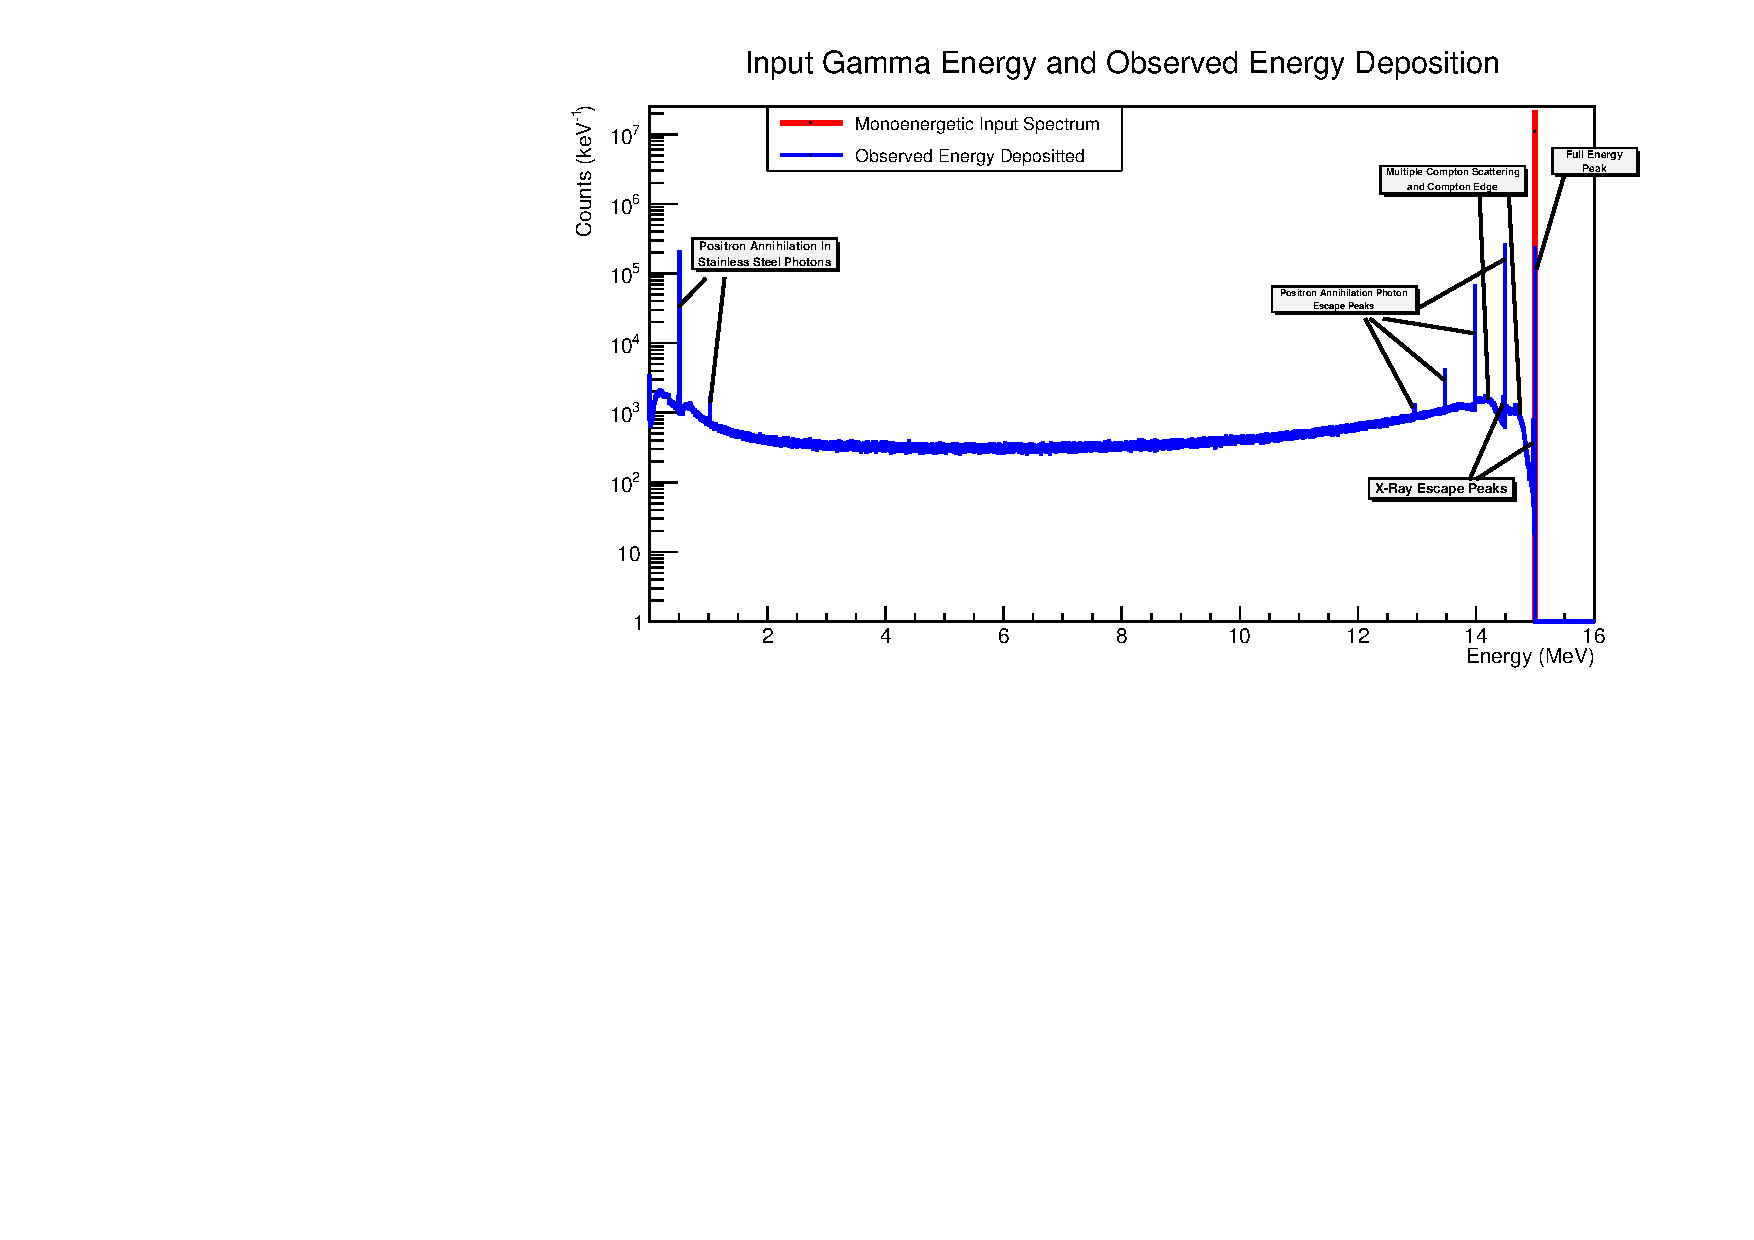
\includegraphics[width=\linewidth]{comparison_pdf}
\caption{(Color Online) A mono-energetic input spectrum and the observed/response energy deposition. Red shows the input gamma rays, blue shows the energy deposited in the detector (the detector's response function.)}
\label{fig-input-vs-response}
\end{center}
\end{figure*}

The spectrum observed in a gamma-ray detector for a given input spectrum is the response spectrum to that input spectrum, if the input spectrum is mono-energetic then the response spectrum is know as the response function. In gamma-ray spectroscopy a frequent goal is to find the input spectrum for an observed response spectrum, this process frequently called decomposition or unfolding. Decomposition is made difficult by a few problems. The first of these problems is the generation of the response functions for the gamma-rays that are present in your input spectrum (for decomposition these functions become the rows of a matrix called the response matrix). It is very difficult measure the response function of a mono-energetic input spectrum. There is almost always background present, and most gamma-ray sources are not mono-energetic. Such a measurement may be possible using a tagged bremsstrahlung facility but, the paucity of such facilities and shielding necessary to screen background radiation would render such an measurement difficult. Another difficulty of decomposition is the nature of the problem to be solved. Decomposition can be expressed mathematically as $\vec{o} = \mathbf{R}\cdot{}\vec{i}$ where $\vec{o}$ is the observed spectrum, $\mathbf{R}$ is the response matrix, and, $\vec{i}$ is the input spectrum. At first glance this could be solved by simple matrix inversion. However, this is made difficult by the response matrix rarely being square, the similarities between response functions causing the matrix to be nearly singular, and the fact that such a procedure can easily result in negative input gamma-ray intensities - a clearly impossible and unphysical result.

\section{Simulation and Generation of the Response Matrices for Large Volume NaI detectors}
%Talk about monte carlo techniques, successes and failings. Talk about Geant4. Briefly talk about the PG4 framework
Monte Carlo simulation techniques help bridge the divide between the theory describing particles interacting with matter and the reality of detecting those interactions. With the explosion of computer power they represent a good method for seeing how a detector will respond to a given input without even building the detector. While they cannot simulate unknown physics, they can simulate the effects of known processes, and even hypothetical processes, for a given particle within a detector. This allows one to build up a picture of how a particle will move through a detector, where and how it will deposit, and even how the ionization and excitation from those energy depositions will resolve. This makes Monte Carlo simulation techniques ideal for, among other things, calculating the response functions and constructing the response matrix for a detector.

A popular package for performing Monte Carlo simulations of physical processes is GEANT4 (GEometry ANd Tracking). GEANT4 is a C++ framework that allows the user to specify in code the geometry that they wish to simulate, the materials it is made of, and the properties of those materials. Then the user can define what the particles to simulate and how they initially move relative to that geometry. Next, the user specifies what physics processes, either individually or as a group, they wish to be included in the simulation and the level of detail of the simulation (below what energy can the simulation ignore a particle for non ``at-rest'' processes, are optical photons generated by energy deposition in a scintillator, etc.) Finally, the user specifies what information they wish to record when the particle interacts in the detector, location, deposited energy, and process type to name a few possibilities. With this complete the user can compile their code and ``throw'' particles into the detector until they have collected adequate statistics to describe what will be seen in the detector.

The Precision Reactor Oscillation and SPECTrum experiment (PROSPECT) has built a lightweight framework on top of GEANT4 (PG4) allowing relatively quick setup of simulations and extraction of data from the simulation. The framework provides, among other things: a simple way of making shells of material around other pieces of material, a simplified primary event generation system, and an already specified and easy to access set of information to extract from particle interactions. These make the framework attractive for simple simulations that are related to the PROSPECT project. As the large volume NaI detectors discussed hereafter were being used to measure the gamma-ray flux that the PROSPECT detector would be immersed in, PG4 was utilized to ease the coding of the simulations needed to find the response matrix for the detector.

\subsection{Geometry and Approximations}
\begin{figure}[h]
\begin{center}
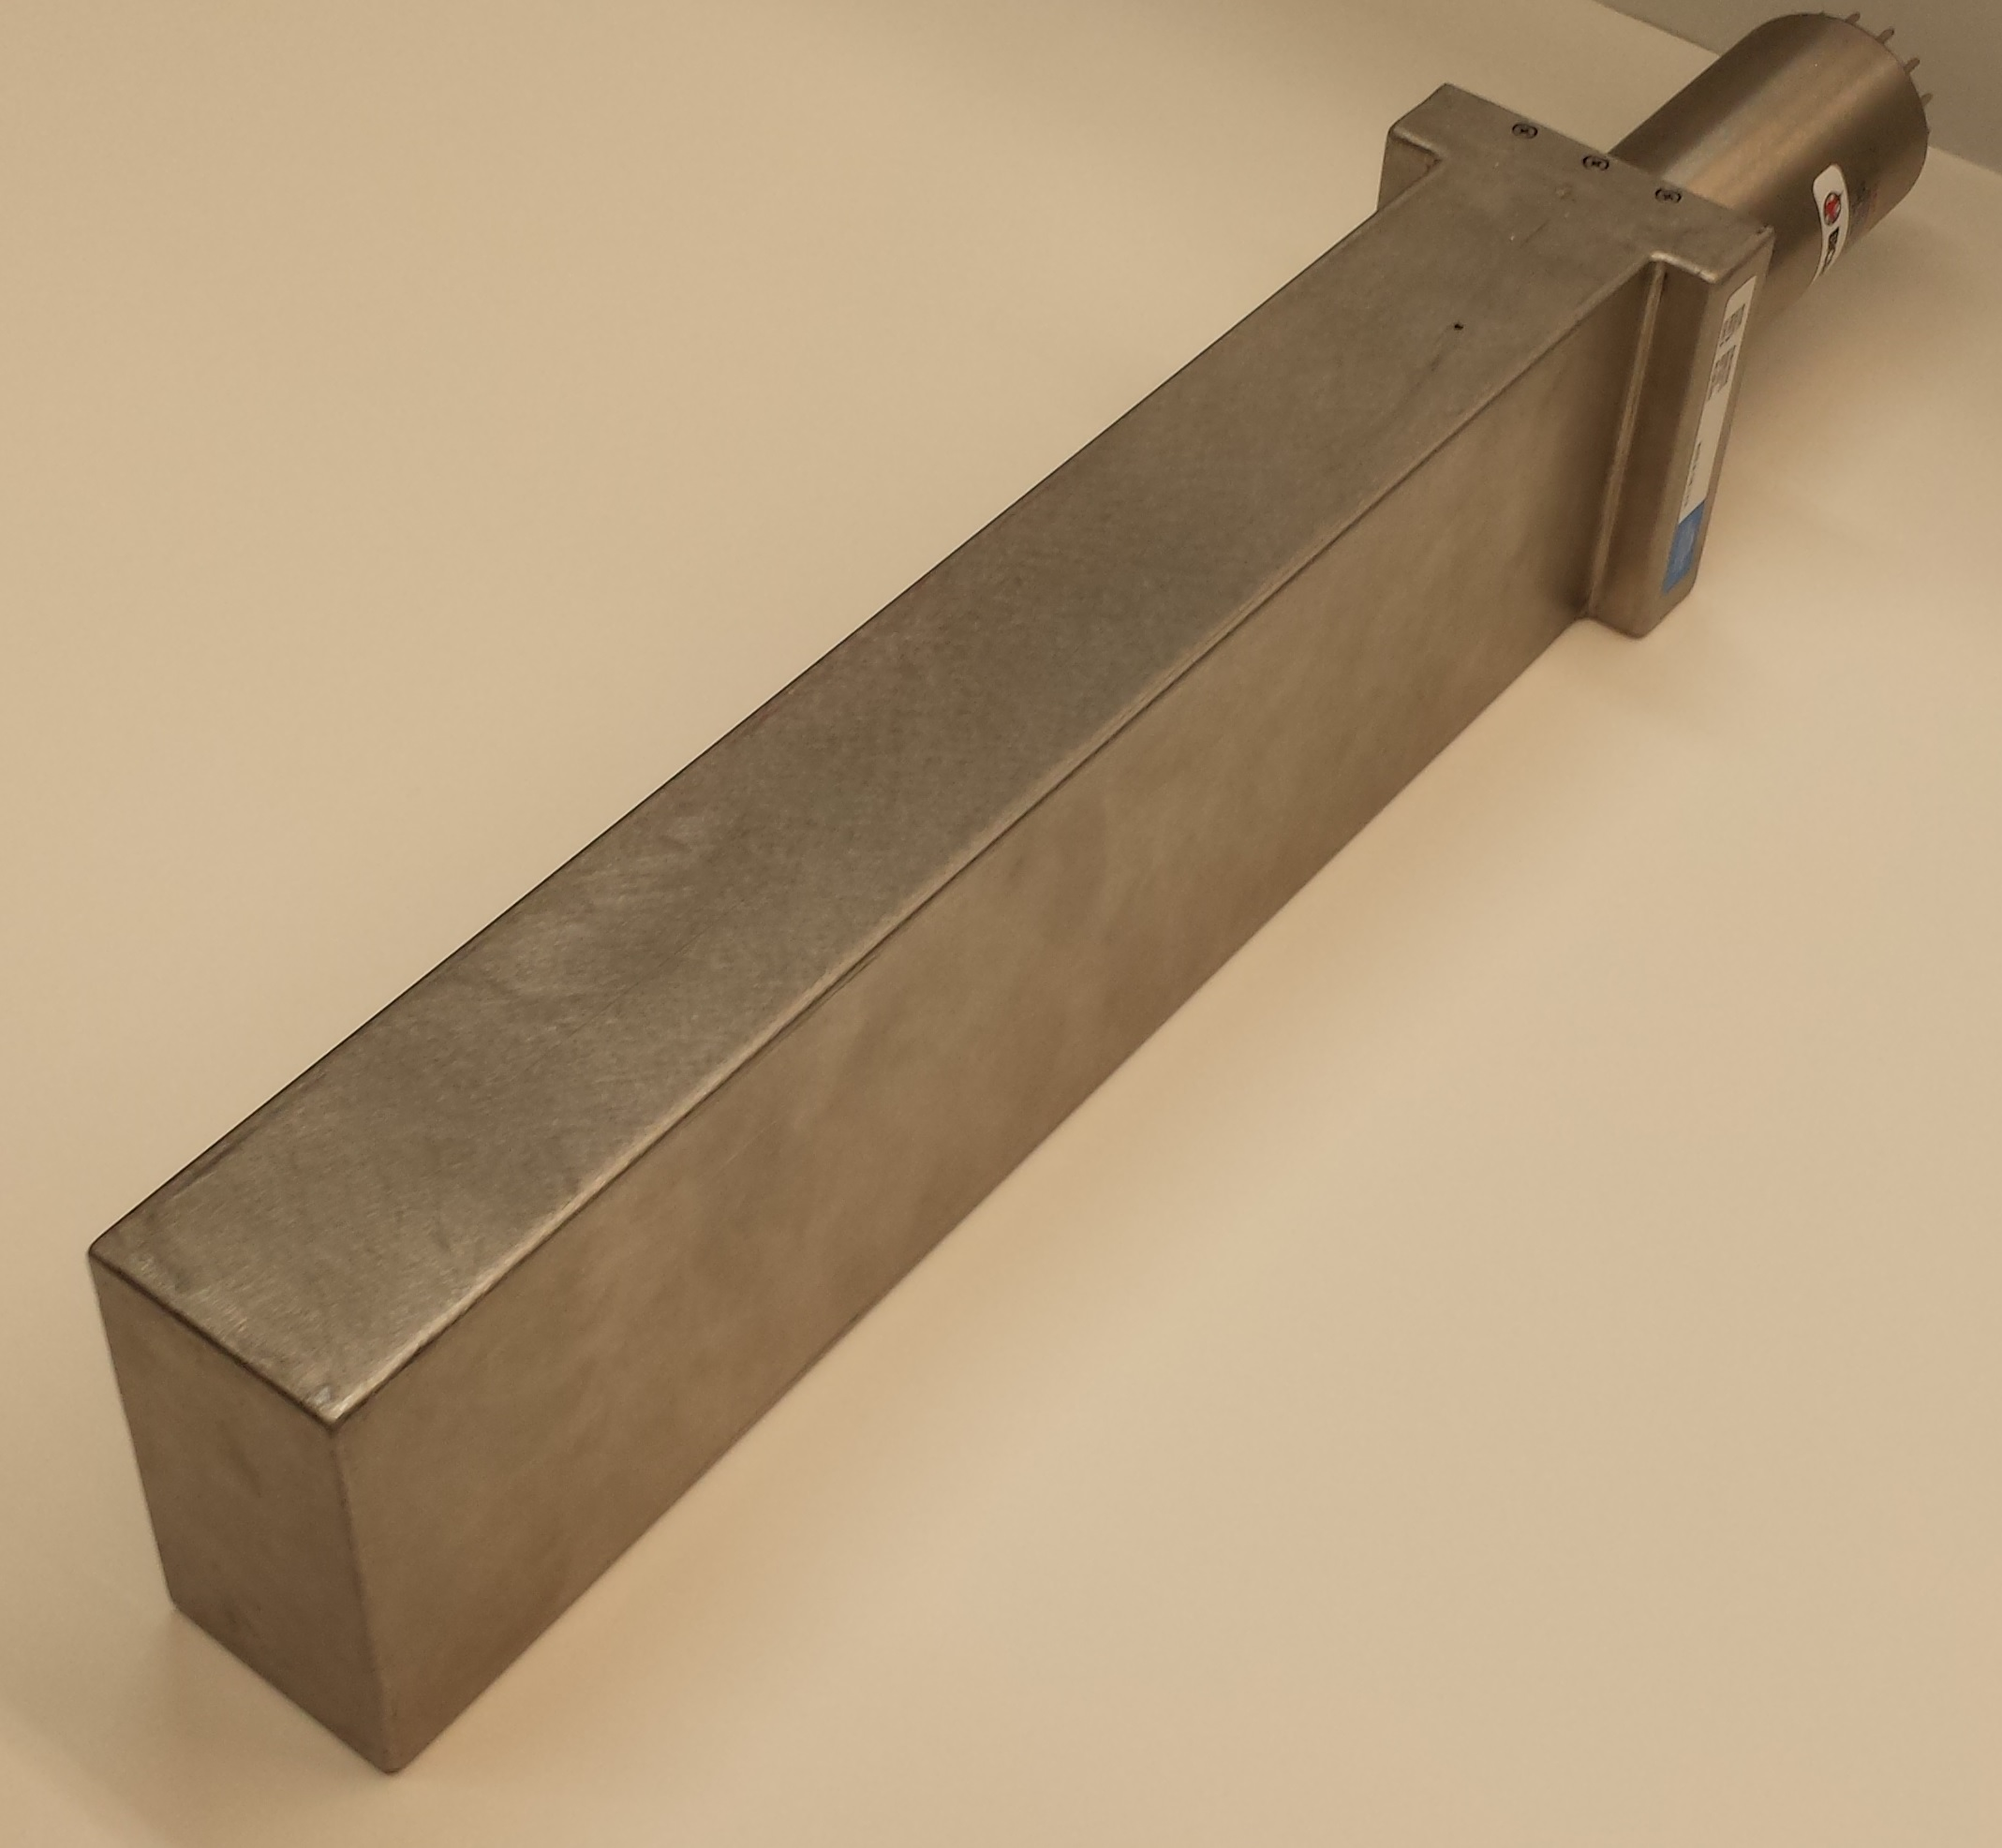
\includegraphics[width=\linewidth]{det_images/three_quarters}
\caption{(Color Online) A three quarters view of the detector to be simulated.}
\label{fig-det-three-quart}
\end{center}
\end{figure}
The large volume NaI(Tl) detectors are fairly simple in their construction. The NaI(Tl) crystal itself is 16in(40.64cm) long, 4in (10.16cm) tall, and 2in (5.08cm) thick. The crystal is surrounded on five sizes by a 0.125in (0.3175cm) thick stainless steel shell. On the sixth side is a small flare to accommodate mounting the Photo-Multiplier Tube (PMT) to the crystal and the PMT itself. This can be seen in Fig. \ref{fig-det-three-quart}.

To simulate the detector a few approximations to its geometry were made: The flare and PMT were omitted, instead the side they occupy was covered in a 0.125in thick layer of stainless steel, the same as the other side of the detector. This omission wons done to drastically simply the construction of the detector geometry and is expected to have a small but noticeable effect on the response to gamma rays approaching from that end of the detector. The effect is small because the volume of PMT is mostly vacuum, which does not scatter gamma rays. However, the lack of this additional inactive mass will cause a smaller 511keV response line from pair production in the shell as well as a smaller Compton scattering continuum due to reduced Compton scattering in the shell. 

Additionally, the corners and edges of the detector were not beveled, instead they were sharp. This made construction of the geometry easier as well as speeding the simulation somewhat because curved edges are more difficult to calculate. This should have minimal impact on the simulated response functions because of the minimal amount and peripheral location of mass added. What minimal effect there is would result in a slightly increased 511keV response and slightly larger Compton scattering continuum due to increased pair production and Compton scattering in the additional stainless steel; however these effects would require careful analysis of response functions to observe.

The final approximations were made in the choice of materials. The NaI crystal did not have a thallium dopant added. This was done because a typical thallium concentration in NaI(Tl) is 0.022mol\% an exceedingly small value that should have little to no noticeable effect on the response functions. Additionally, the grade of stainless steel for the shell was not known. Because of this the stainless steel chosen in simulation was SAE 444; chosen for its corrosion resistance and common use in cladding applications, it seemed a likely candidate and as the composition of many stainless steels are similar it should have no noticeable impact on the simulated response functions.

The final geometry simulated with a single simulated event can be seen in Fig. \ref{fig-det-geom-sim}.
\begin{figure}[h]
\begin{center}
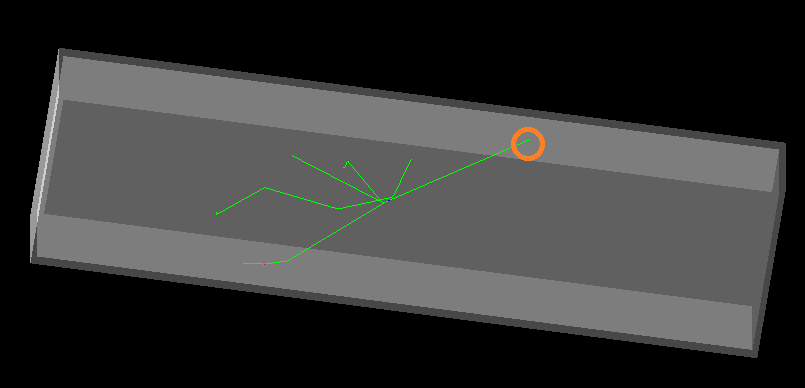
\includegraphics[width=\linewidth]{geometry}
\caption{(Color Online) A view of the simulated geometry with a single 15.0MeV gamma ray interacting. The translucent outer grey cuboid is the stainless steel cladding, the inner cuboid is the NaI crystal. The origin of the gamma ray is circled in orange. Gamma-ray tracks are green, electron tracks are red, and positron tracks are blue.}
\label{fig-det-geom-sim}
\end{center}
\end{figure}

\subsection{Event Generation}
Because the simulation geometry of the detector has 3 symmetry planes, simulation of an isotropic gamma flux can be simulated throwing gammas in from only three of the six sides. To facilitate this a mono-energetic gamma-ray thrower was developed to throw an effectively isotropic flux into the detector from a chosen side. During setup the user chooses a side and gamma-ray energy and during simulation, for every event to be simulated the event generator randomly selects a point on the surface of that side and a point within the volume of the detector and its stainless steel shell. It then creates a gamma-ray with the selected energy at the surface point traveling towards the point within the volume.

\subsection{Information Recorded}
PG4 makes a great deal of information easily available for recorded in these simulations: exact locations of each interaction, type of each interaction, energy deposited in the interaction, etc. The type of each interaction was ignored because, for the interactions expected, the type would have no effect on the scintillation light yield. While knowing the interaction locations can be useful since the light collected is somewhat dependent on the location the light is generated from it was ignored. Ignoring interaction locations drastically simplified the collection of data and made a difficult simulation of light generation and collection unnecessary. In the end, only the sum energy deposited in all the interactions of a single event was recorded in a histogram for each event. This dramatically simplified the analysis and use of the simulation data.

\subsection{Response Functions}
\begin{figure}[h]
\begin{center}
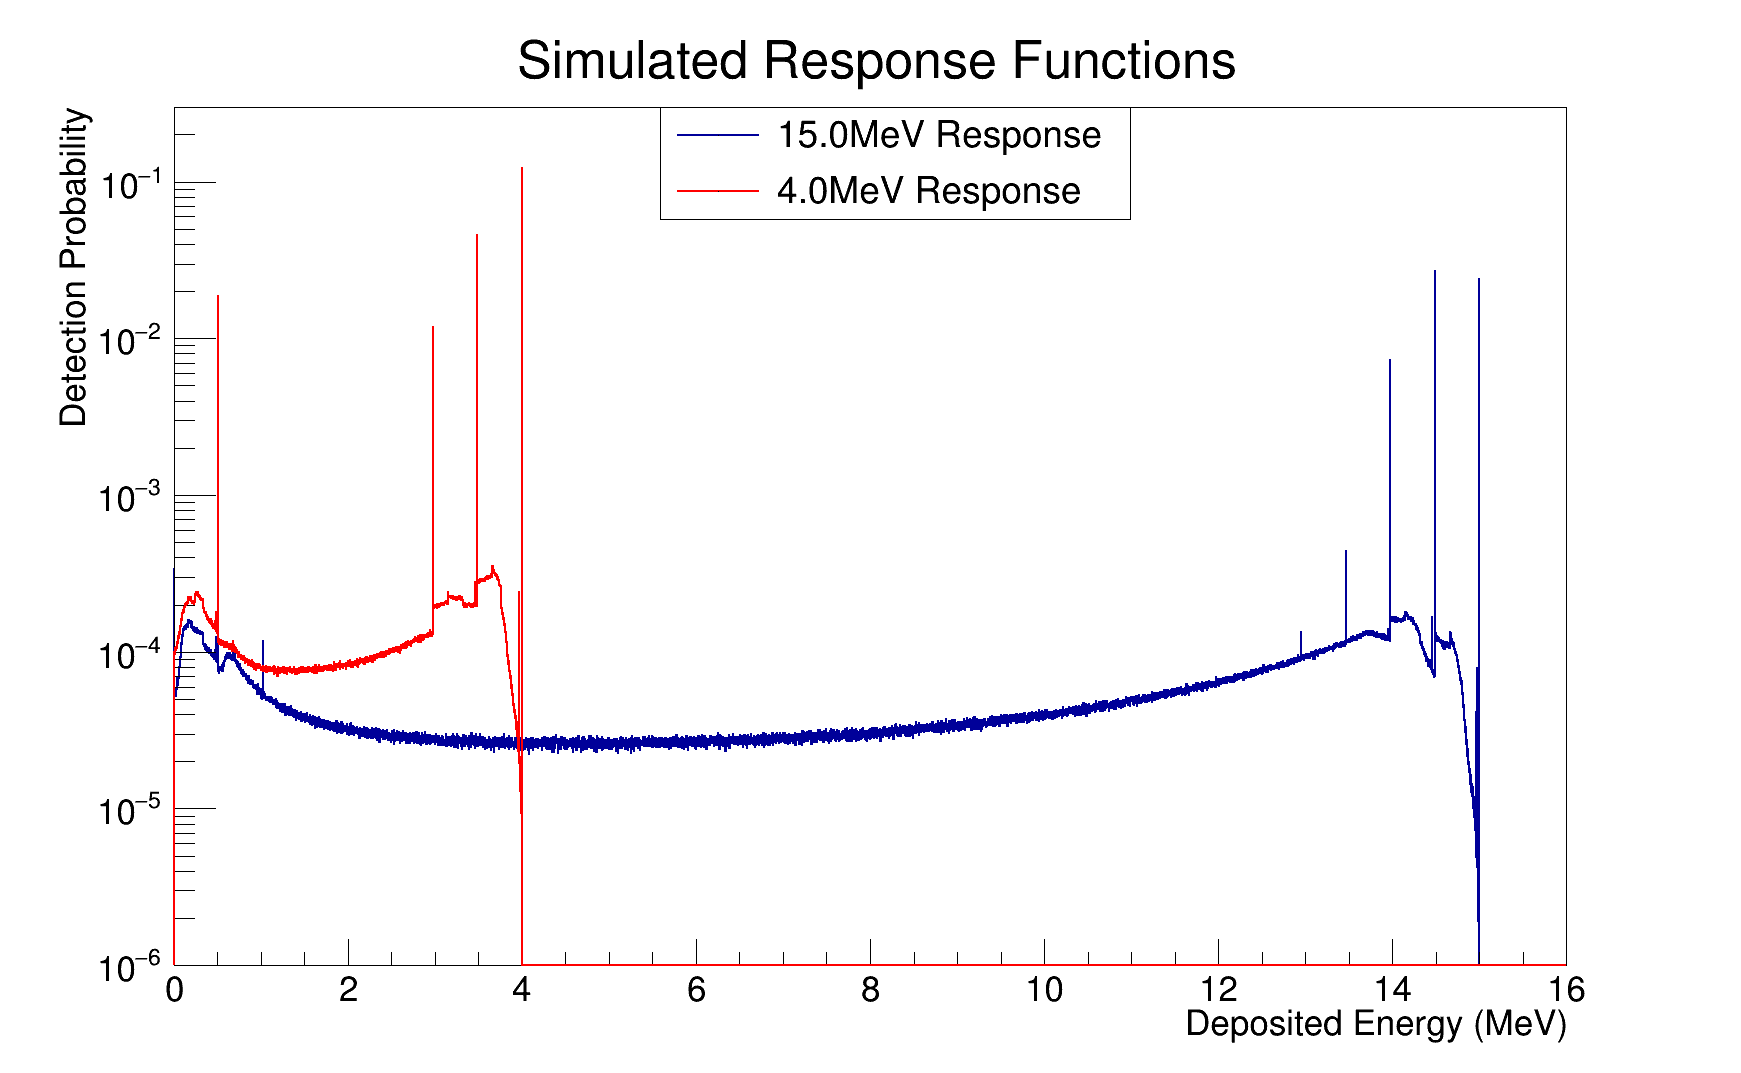
\includegraphics[width=\linewidth]{response_png}
\caption{(Color Online) Two simulated response functions for isotropic flux of gamma-rays at 15.0MeV and 4.0MeV. The peak at 0.511MeV is due to pair production in the shell of the detector and one of the positron annihilation photons entering the detector. The peak at 1.022MeV is caused in a similar manner by double pair production, wherein one of the particle produced in the first pair production radiates a photon via the bremsstrahlung process which in turn undergoes pair production. The peaks visible at 3.49MeV, 2.98MeV, 14.49MeV, and 13.98MeV are caused by the pair production within the scintillator and one or both of the annihilation photons escaping the scintillator without being detected. The peaks at 13.47MeV and 12.96MeV are produced in a similar manner via double pair production within the scintillator material. Finally, the peaks at 4.0MeV and 15.0MeV correspond to the full energy of the gamma ray being deposited within the scintillator crystal.}
\label{fig-resp-func}
\end{center}
\end{figure}
For each response function events striking each detector side were simulated. To ensure good counting statistics and even coverage of each side, the number of events was chosen to be 160000 gamma rays per square inch of the side. Once each side was simulated the resultant histograms were normalized so that the y-axis corresponded to the probability that a given amount of energy would be deposited in a given event. The responses for the three sides were then summed after being weighted by the sides relative surface area, giving the response function for the detector corresponding to an isotropic flux. Two such response functions are shown in Fig. \ref{fig-resp-func}. This process we performed for gamma-ray energies between 10keV and 15.0MeV, every 10keV.

The next step is to make these response functions realistic. Because detectors do not perfectly record the amount of energy deposited within then but instead have some ``fuzziness'' in their response to identical energy deposits it is necessary to introduce this fuzziness by convoluting the simulated detector response function with a Gaussian function describing the width of peaks in the detector (shown in Eq. \ref{eqn-gauss-width}).

\begin{align}
W(E-\lambda{}, E) \propto e^{\frac{-(E-\lambda{})^2}{2*\sigma{}^2(E)}}
\label{eqn-gauss-width}
\end{align}

Here $E$ is the observed energy in the output spectrum, $\lambda{}$ is the input energy of the convolution which is being summed across, and $\sigma{}^2(E)$ was fitted to data from the detectors using the form $\sigma{}^2(E) = A + B*E$ (with $A$ and $B$ fitted parameters.) The result of this convolution can be seen in Fig. \ref{fig-convol-effect}.

\begin{figure}[h]
\begin{center}
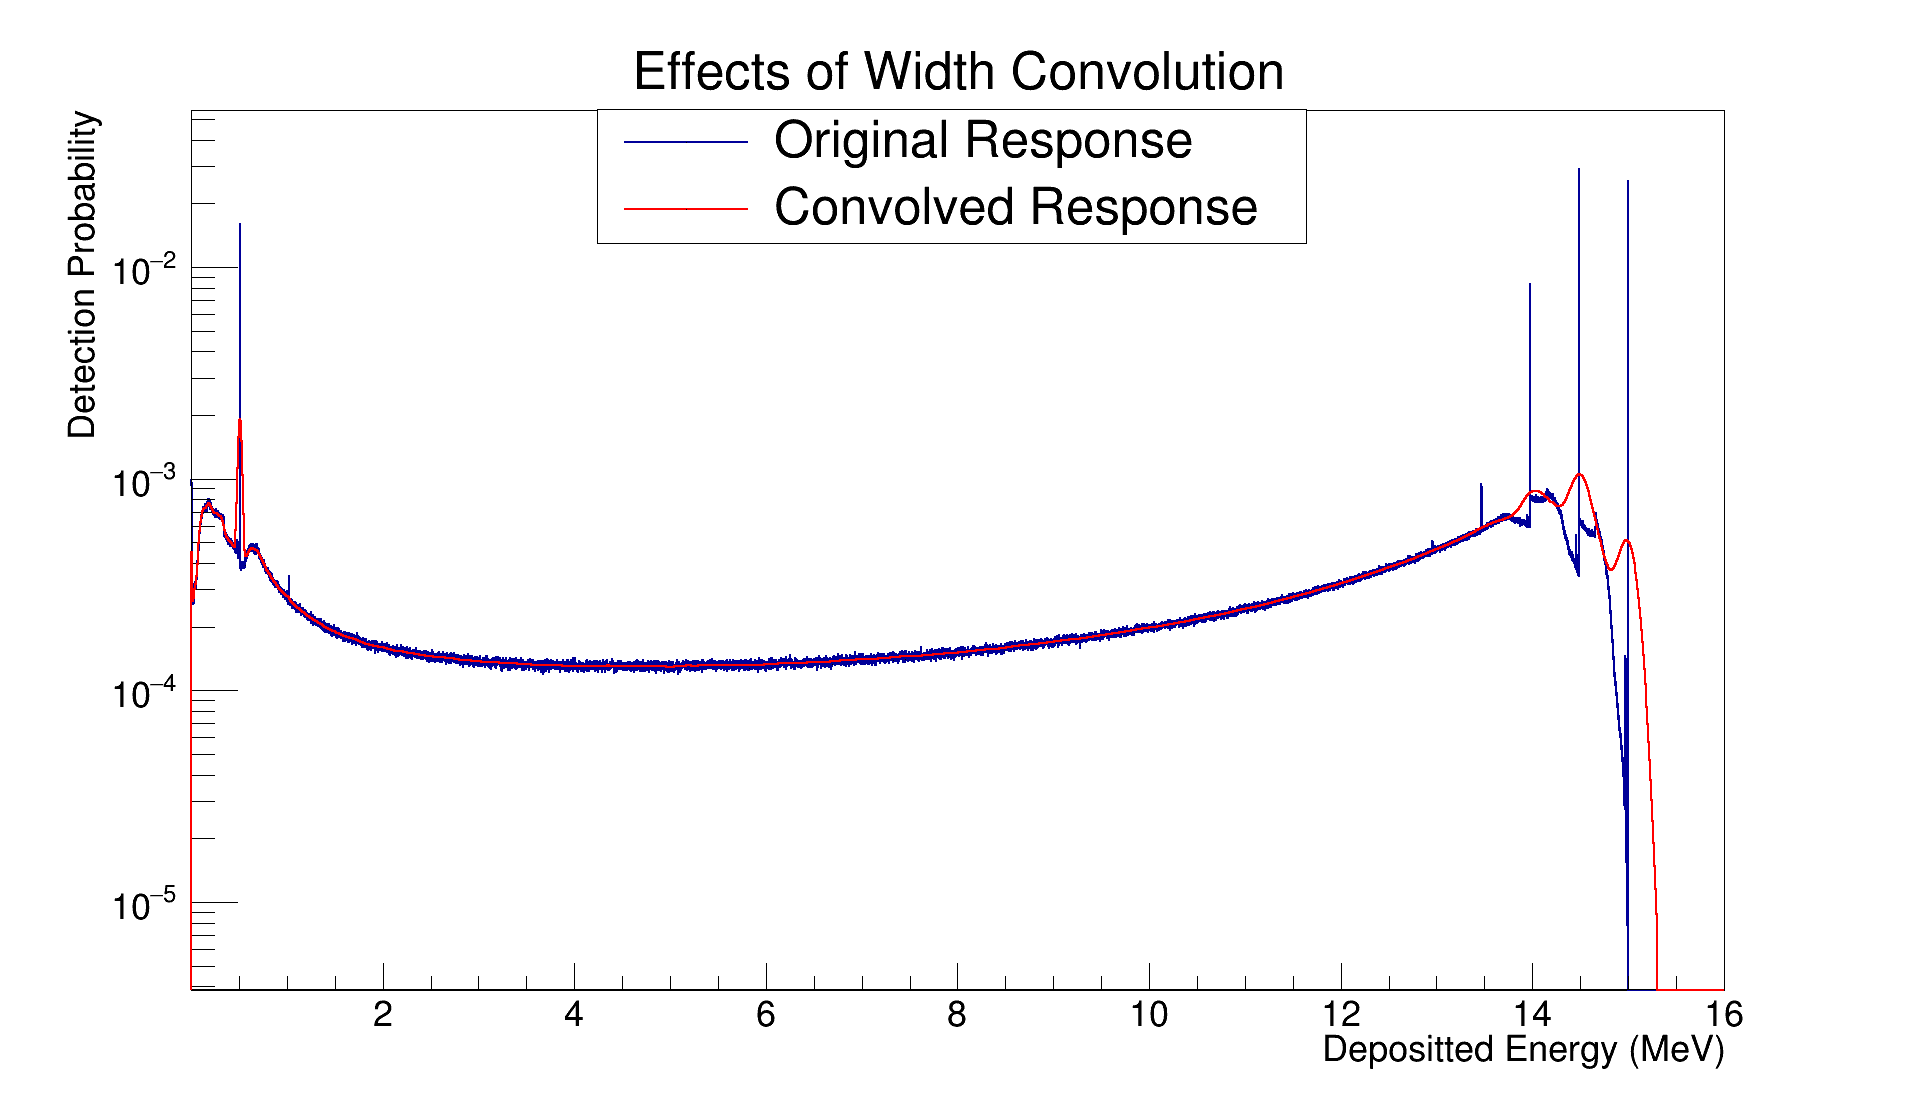
\includegraphics[width=\linewidth]{convolve_diff_png}
\caption{(Color Online) A plot showing the effect width convolution has on the simulated response function. Blue shows the original simulated response function and red shows the response function after convolution.}
\label{fig-convol-effect}
\end{center}
\end{figure}

\subsubsection{Convolution Implementation}
The equation describing the discretized convolution used to make the simulated response function realistic can be seen in Eqn. \ref{eqn-convolution}.

\begin{align}
C(E) = \frac{\sum_{\lambda{}=0}^{E_{Max}}  e^{\frac{-(E-\lambda{})^2}{2*(A + B*E)}} * SR(E)}{\sum_{\lambda{}=0}^{E_{Max}}  e^{\frac{-(E-\lambda{})^2}{2*(A + B*E)}}}
\label{eqn-convolution}
\end{align}

Here $SR(E)$ is the simulated response function to be convolved, $A$ and $B$ are parameters fitted to data, and $E_{Max}$ is the maximum energy of the output spectrum $C(E)$. The denominator is necessary to ensure the total normalization of the output spectrum stays the same.

Under normal circumstances discrete convolution can be performed quickly due to its similarity to the discrete Fourier transform allowing one to use an algorithm based on the fast Fourier transform (FFT), giving a time proportional to $n*lg(n)$ instead of $n^2$ (where n is the number of bins in the input spectrum.) Unfortunately, when the Gaussian function to be convolved is dependent on both $(E-\lambda{})$ \emph{and} $E$ the path to this shortcut is unclear and was not able to be used. Instead two different techniques were used to speed the convolution. The first technique was the realization that once $\frac{(E-\lambda{})^2}{2*(A + B*E)} > 8$, the Gaussian is very small and can be neglected, allowing somewhat narrower limits on the inner loop. The other technique exploited the fact that the convolution of each response function was independent of the convolution of other response functions and so the convolutions could be performed in parallel, granting another constant factor speed up.

Once the functions have all been convolved with realistic resolutions they were placed in a matrix, for a specific detector and run this is shown in Fig. \ref{fig-resp-mat}

\begin{figure*}[t]
\begin{center}
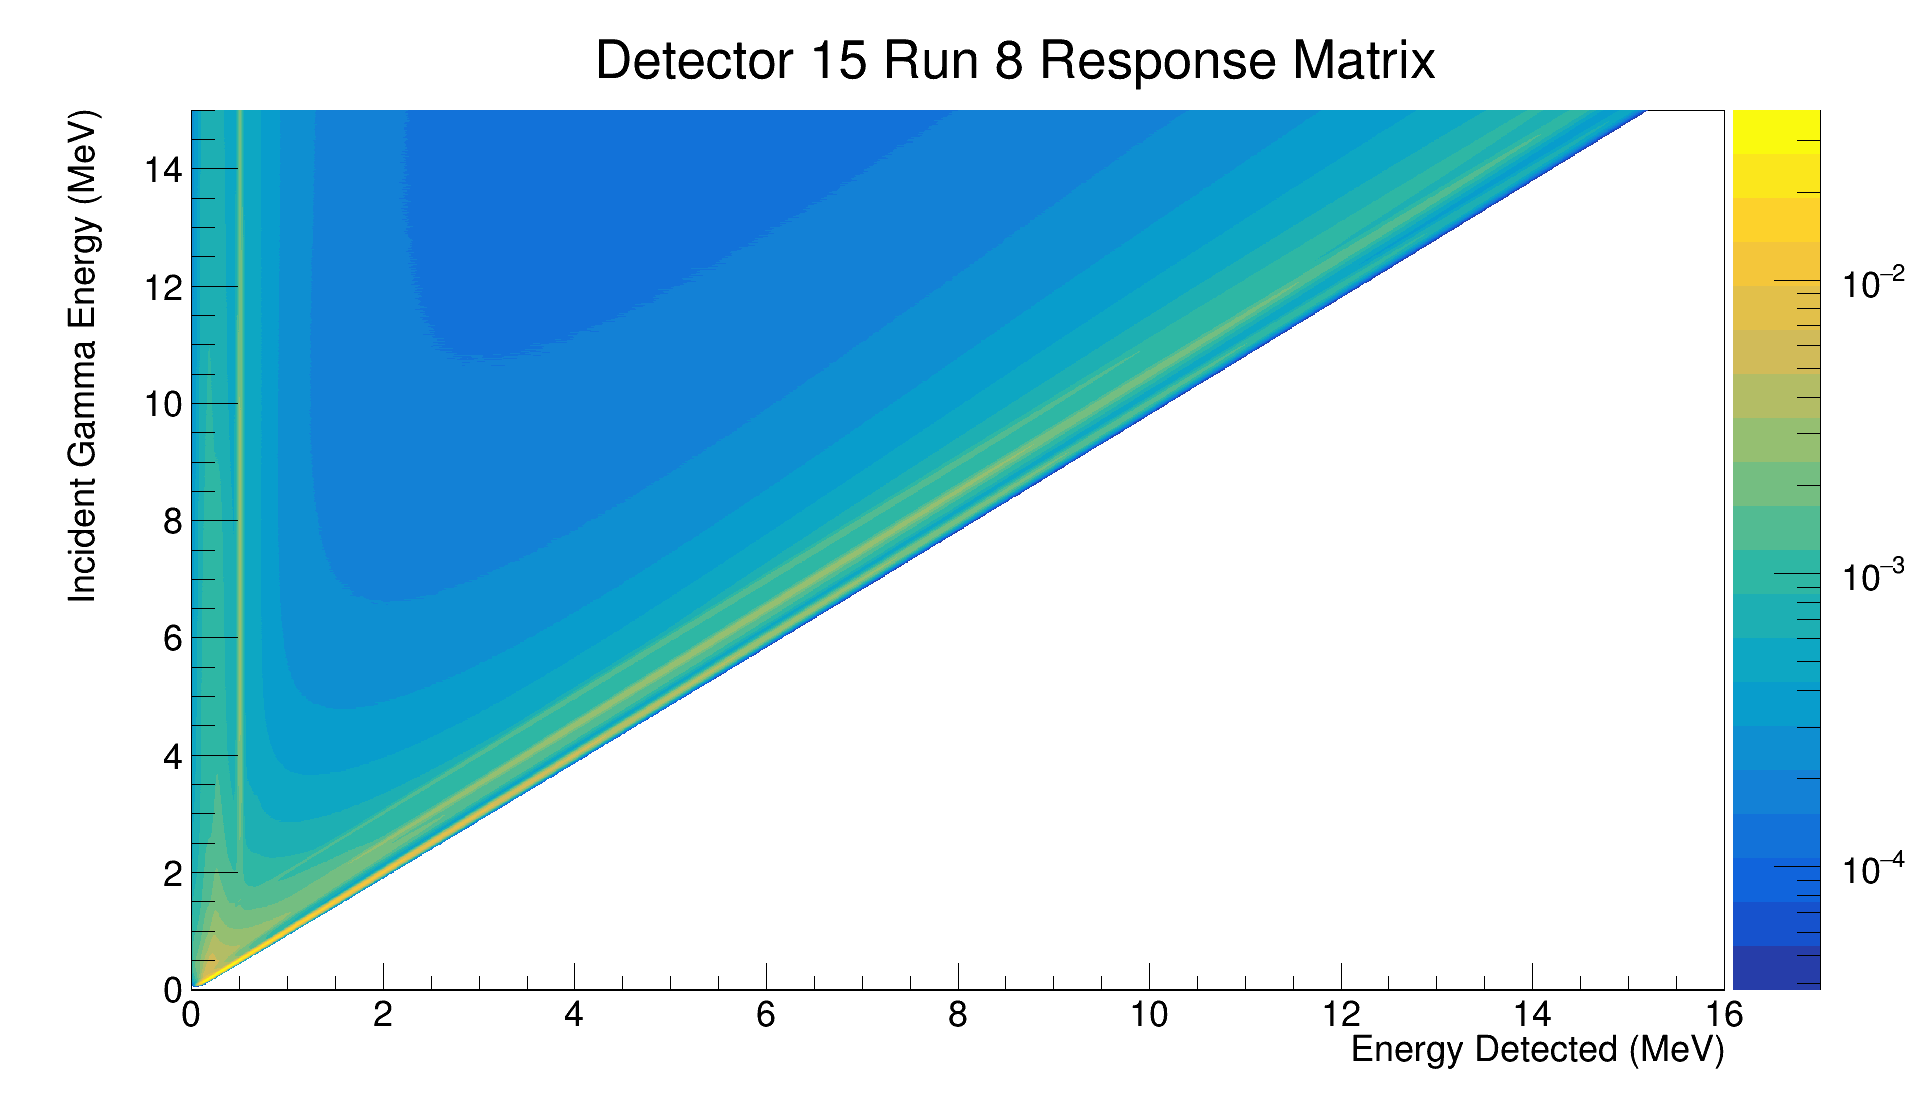
\includegraphics[width=\linewidth]{resp_mat_png}
\caption{(Color Online) The response matrix determined for a particular detector and run. Color shows the probability of detecting a particular amount of energy for a given incident energy.}
\label{fig-resp-mat}
\end{center}
\end{figure*}

\section{Decomposition}
Decomposition is the solution of the inverse problem converting the observed spectrum of gamma rays into the incident spectrum of gamma rays. The process is quite difficult for several reasons: Solutions are not unique and the set can contain solutions that are physically unreasonable, for instance one may obtain negative gamma-ray fluxes incident upon the detector in a naive solution, clearly unreasonable. Inverse problems such as this are known as \emph{ill-conditioned} or \emph{ill-posed}\cite{TainOtt2007}. This difficulty is further compounded by the inversion of the response matrix. Because response matrices are rarely square so the naive matrix inversion may not even be possible. When the naive inversion is possible another problem can rear its head. Because response functions for nearby incident energies can have substantial self-similarity, the response matrix can be singular or close to singular. This in turn either prevents the finding of the appropriate inverse entirely, or it can cause problems in the computation because of the finite precision of computer arithmetic.

\subsection{The Algorithm}
Fortunately there are numerous methods other than the direct matrix inversion and multiplication. In Ref. \cite{TainOtt2007} Tain and Ott discuss several methods for the decomposition of the spectra seen in total absorption gamma-ray spectroscopy, a problem that is essentially identical to what is needed to be solved in this case. Testing of the methods presented, LR, maximum entropy, and expectation maximization showed that iterative expectation maximization gave the best results for this particular problem, having excellent numerical stability and producing positive definite output histograms. Eqn. 21 in Ref. \cite{TainOtt2007} describes the expectation maximization method; however, as it is written there are problems with the indices, Eqn. \ref{eqn-decomposition} below gives the method in a corrected form, which was derived from the original version of the method given in Ref. \cite{lucyAstro1974}. A psuedo-code implementation of the algorithm is given in Alg. \ref{alg_decomp}

\begin{align}
f_{\mu}^{(s+1)} = \frac{1}{\sum\limits_{j}R_{\mu{}j}} \sum\limits_{i}\frac{f_{\mu{}}^{(s)} R_{\mu{}i}d_i}{\sum\limits_{\alpha}R_{\alpha{}i}f_{\alpha}^{(s)}}
\label{eqn-decomposition}
\end{align}
Here $m$ is the number of response functions, $n$ is the number of data bins, $R$ is the matrix of response functions $(m \times n)$, $d$ is the input spectrum vector $(n \times 1)$, and $f^{(s)}$ is the decomposed spectrum in the $i^{th}$ iteration $(1 \times m)$. $f^{(0)}$ can be chosen to be any $(1 \times m)$ vector of values whose elements are greater than 0; however, good choices will significantly reduce the number of iterations required to obtain convergence.

\begin{figure}[h]
\begin{center}
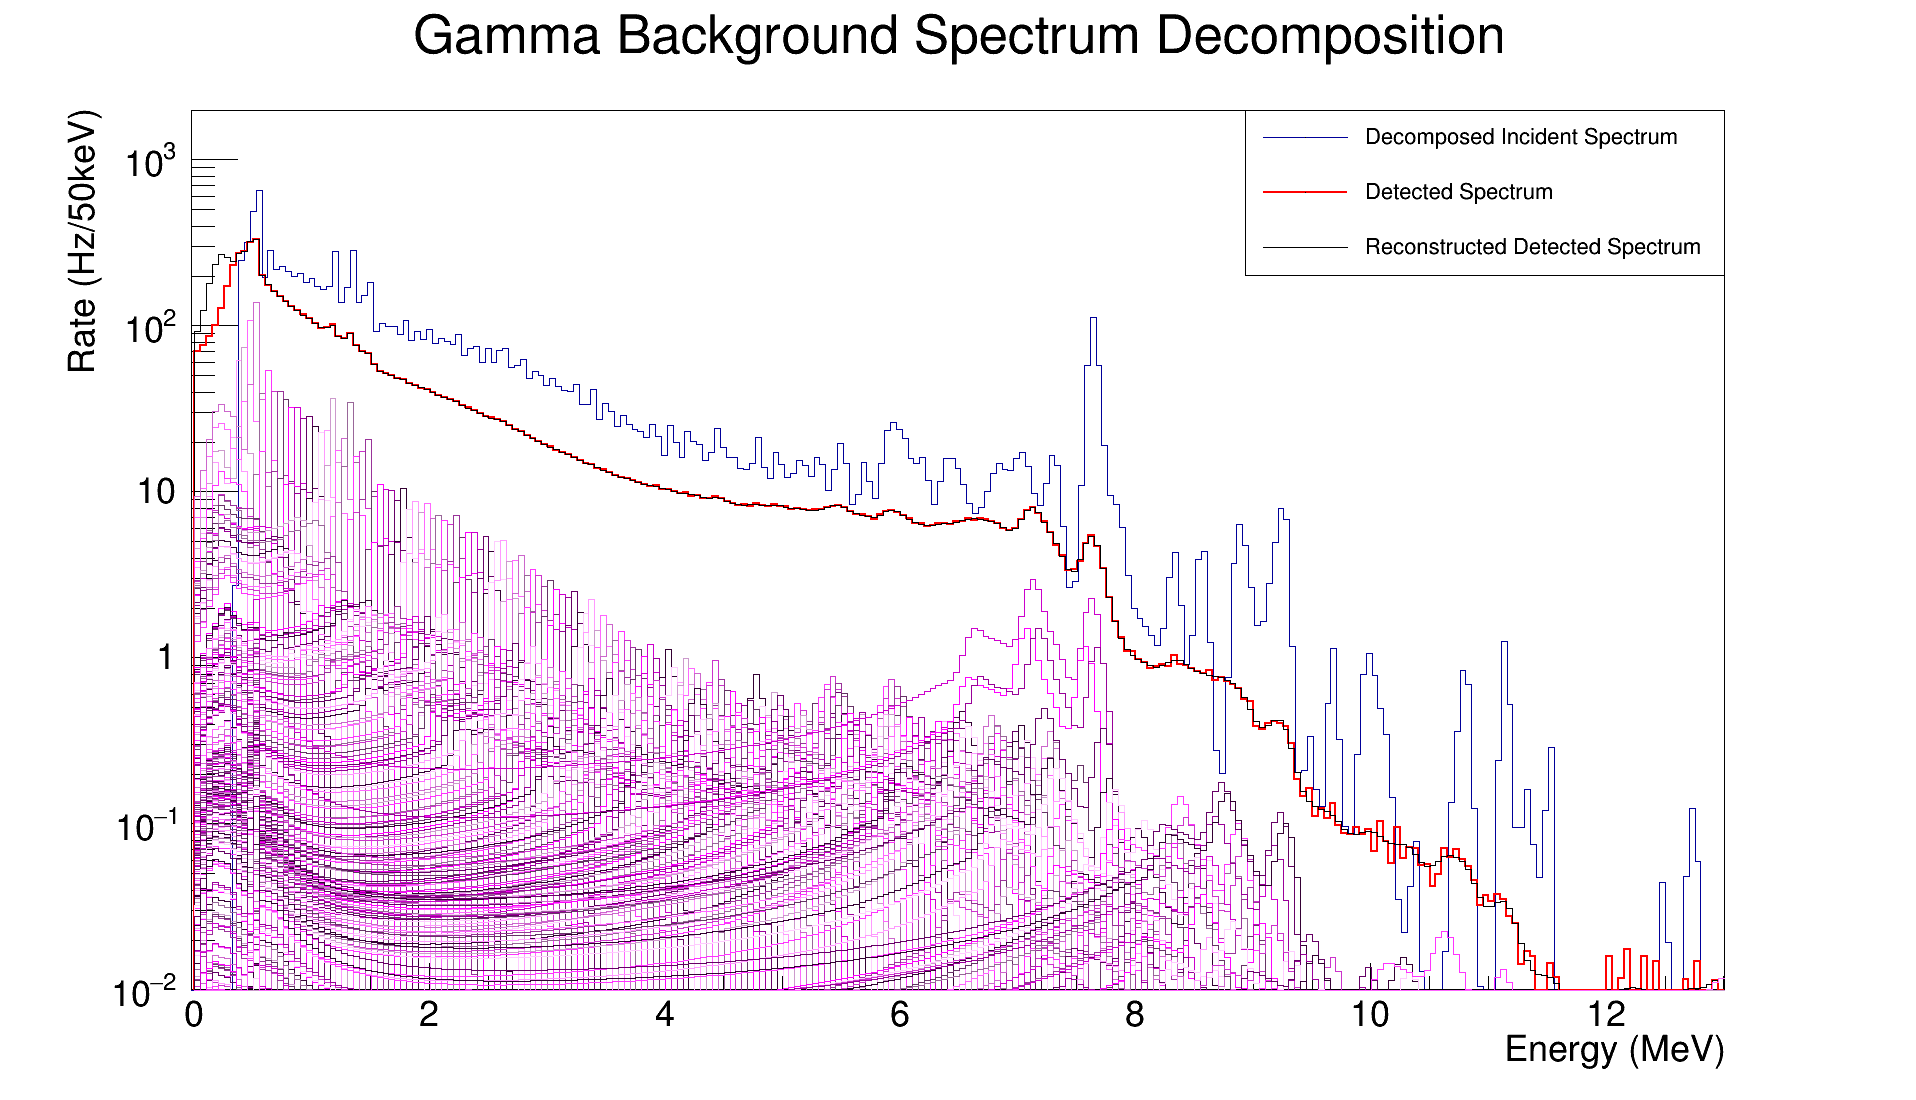
\includegraphics[width=\linewidth]{fit_plot}
\caption{(Color Online) A low resolution decomposition of a spectrum taken in a room seven meters from the High Flux Isotope Reactor core. The blue line is the deduced spectrum incident on the detector, the red line is the spectrum observed in the detector, the black line is the reconstruction of the observed spectrum from the decomposed parameters, and all the other lines represent the weighed response functions that must be summed to obtain the black line. Present in this spectrum is: $^{60}$Co (from activation), $^{40}$K (from concrete), down-scattered high energy gamma rays, and several lines resulting from neutron capture on common materials in the area.}
\label{fig-low-res-decomp}
\end{center}
\end{figure}

\begin{algorithm}[H]
\caption{Decomposition algorithm for converting observed spectra into incident spectra for a given response matrix. $\odot$ is the element-wise multiplication operator and $\oslash$ is the element-wise division operator. $m$ is the number of response functions, $n$ is the number of data bins.}\label{alg_decomp}
\begin{algorithmic}
\Procedure{DecomposeSpectrum}{$s, R, f^{(0)}, L, \tau{}$}
\BState \textbf{Input}:
\State $s \gets \text{Input spectrum;}$ \COMMENT{$s_j \geq 0$; $\sum\limits_{j=0}^{n}s_j > 0$}
\State $R \gets \text{Repsonse matrix;}$ \COMMENT{$\sum\limits_{j=0}^{m}R_{\mu{}j} > 0$ and $\sum\limits_{j=0}^{n}R_{j\mu{}} > 0$}
\State $f^{(0)} \gets \text{Initial guess;}$ \COMMENT{$f^{(0)}_j > 0$}
\State $L \gets \text{Convergence Limit;}$ \COMMENT{$L > 0$}
\State $\tau \gets \text{Value Threshold For Convergence Test;}$ \COMMENT{$\tau > 0$}
\BState \textbf{Start}:
\State $T \gets R^T$
\State $r \gets \sum\limits_{j}R_{\mu{}j}$
\State $d \gets \textit{False}$
\For{$i \gets 0$; $!d$; $i \gets i+1$}
\State $c \gets T \cdot f^{(i)}$
\State $m \gets s \oslash c$
\State $\Gamma \gets R \cdot m$
\State $f^{(i+1)} \gets f^{(i)} \oslash r \odot \Gamma$
\State $d \gets$ \Call{TestConvergence}{$f^{(i)}, f^{(i+1)}, L, \tau{}$}
\EndFor
\State \Return{$f^{(i+1)}$}
\EndProcedure
\end{algorithmic}
\end{algorithm}

Tain and Ott describe a procedure to determine how many iterations to perform based on obtaining a particular $\chi{}^2$ value. It was found that this method produced poor fits to the observed spectrum and a more stringent limit on the number of iterations was developed. This method compares the calculated incident spectrum at at the end of the iteration with the calculated incident spectrum at the beginning of the iteration. All bins whose contents are above some minimum threshold (to prevent fluctuations due to finite numerical accuracy from preventing convergence) are compared and if any of their fractional differences is greater than a fixed convergence threshold, then another iteration is required. This method forces far more iterations and produces excellent fits to the input spectrum. Typical values chosen for the minimum threshold and convergence threshold were $10^{-6}$ and $5.0\times{}10^{-3}$ respectively. Pseudo-code for this method of convergence can be found in Alg. \ref{alg_conv}

\begin{algorithm}[H]
\caption{Convergence testing algorithm for decomposition.}\label{alg_conv}
\begin{algorithmic}
\Function{TestConvergence}{$f^{(i)}, f^{(i+1)}, L, \tau{}$}
\BState \textbf{Input}:
\State $f^{(i)} \gets \text{Decomposition vector before iteration i}$
\State $f^{(i+1)} \gets \text{Decomposition vector after iteration i}$
\State $L \gets \text{Convergence Limit }$
\State $\tau \gets \text{Value Threshold For Convergence Test}$
\BState \textbf{Start}:
\For{$j \gets 0$; $j<Length(f^{(i)})$; $j \gets j+1$}
\State $cc \gets \abs{\frac{2 \paren{f^{(i+1)}_j - f^{(i)}_j}}{f^{(i+1)}_j + f^{(i)}_j}}$
\If{$f^{(i+1)}_j > \tau$ and $f^{(i)}_j > \tau$ and $cc > L$}
\State \Return{$\textit{False}$}
\EndIf
\EndFor
\State \Return{$\textit{True}$}
\EndFunction
\end{algorithmic}
\end{algorithm}

A sample of Alg. \ref{alg_decomp} with the convergence criteria of Alg. \ref{alg_conv} being used on low resolution input data can be seen in Fig. \ref{fig-low-res-decomp}.

\subsection{Observations}
The implementation and use of this decomposition algorithm comes with several notes of caution and opportunity. Several observations of possible problems, confounding factors, expanded usage, and performance enhancement are described below.

\subsubsection{Pitfalls}
Caution in choice of peak widths that are convolved in the response functions used by this decomposition algorithm is necessary. If the widths chosen are too narrow, peaks formed by a single incident energy will show as several close energies striking simultaneously, as can be seen in Fig. \ref{fig-low-res-decomp} around $7.6$MeV. Conversely, if the chosen width is too broad then the calculated incident spectrum will contain no peaks in the appropriate regions, instead the algorithm will ``settle'' for fitting the average behavior of the spectrum. This can be seen in Fig. \ref{fig-low-res-bad-decomp}, particularly in the $1.0$ MeV to $1.5$ MeV region where the fitted spectrum shows a line through three peaks. While neither extreme is desirable, too-narrow response functions are substantially more desirable than too-wide response functions. The resulting decomposition with too-narrow responses will show the direction of the correction needed and will contain a spectrum broadly similar to a decomposition with perfect peak widths. Additionally, the peak widths seen in such a decomposition can assist in correcting the peak widths in the response functions.

\begin{figure}[t]
\begin{center}
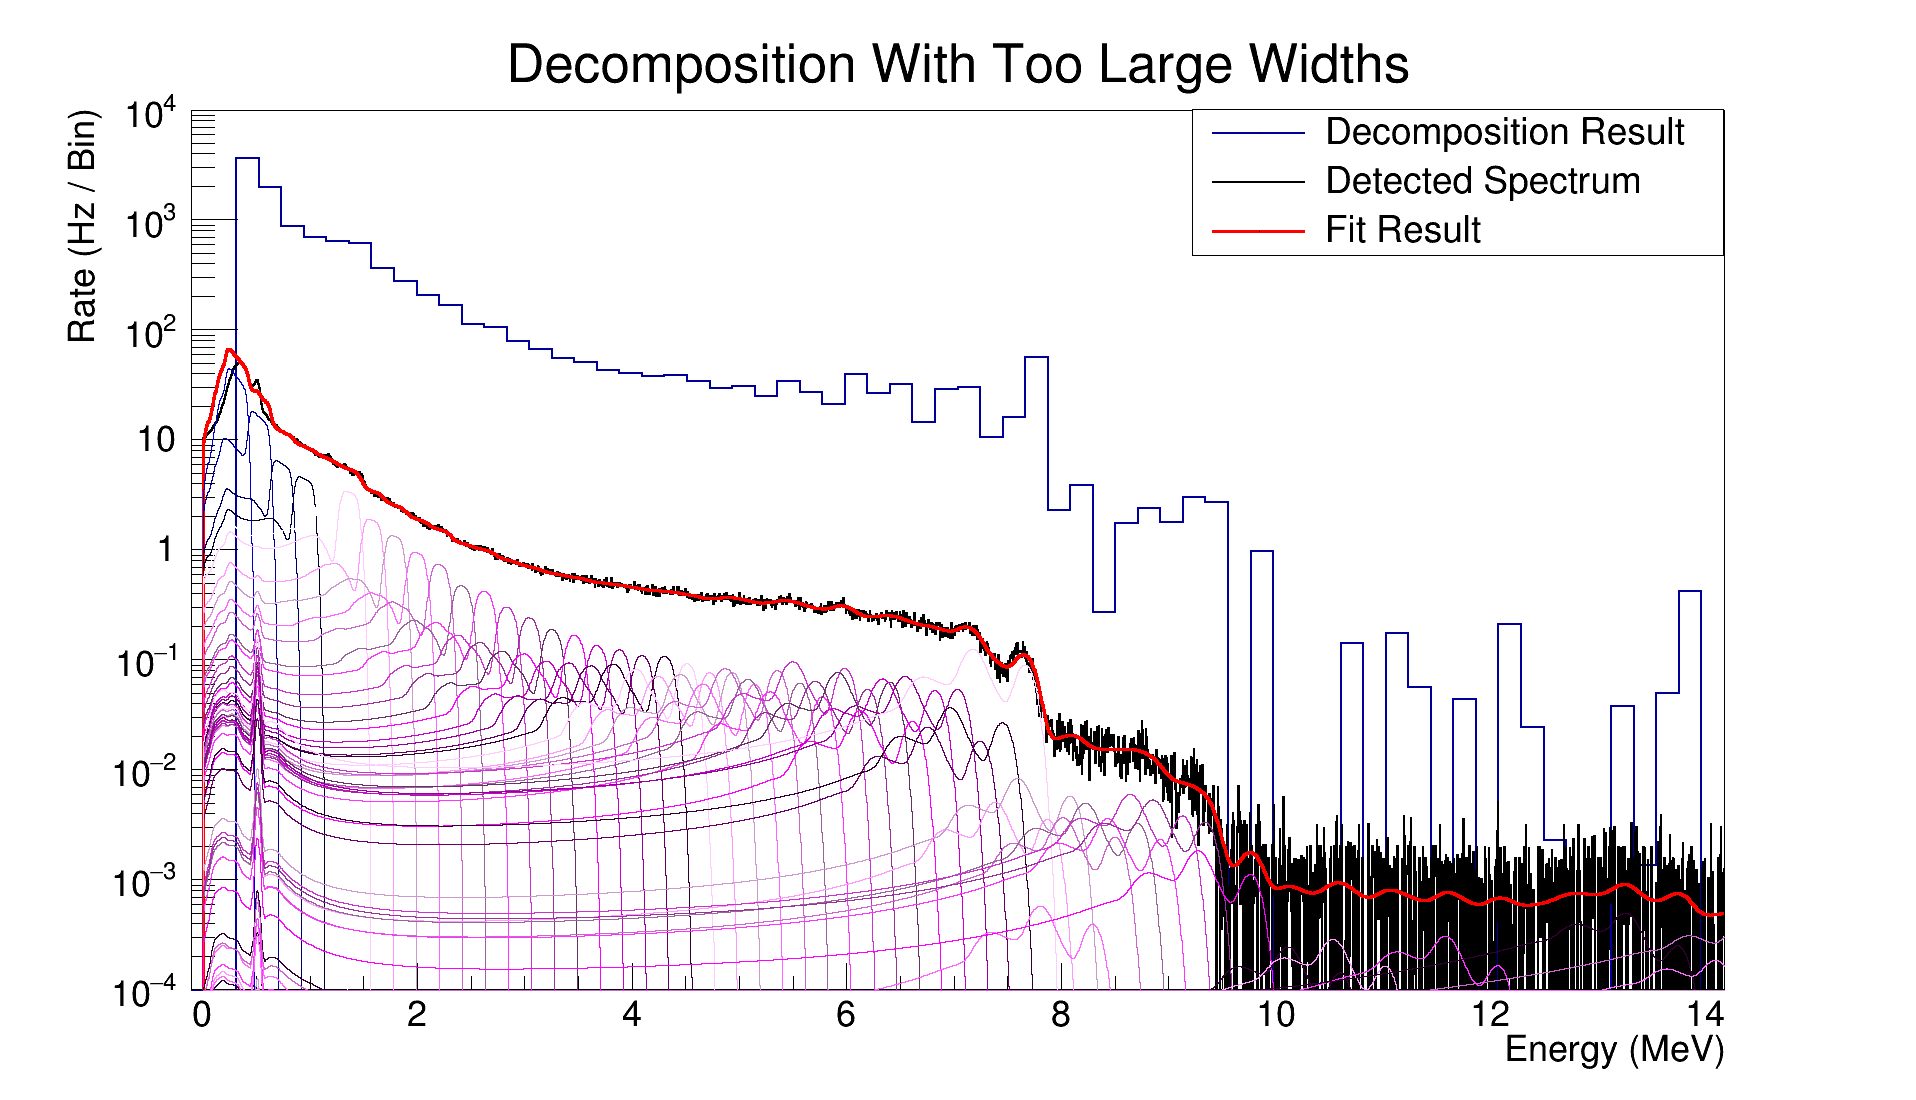
\includegraphics[width=\linewidth]{fit_plot_bad}
\caption{(Color Online) A decomposition of the same spectrum as Fig. \ref{fig-low-res-decomp} with the same meanings and colors; however, the convolved widths of the response function have been set far too large in the low energy regime, demonstrating the peril of such a mistake.}
\label{fig-low-res-bad-decomp}
\end{center}
\end{figure}

Another possible issue in using this algorithm is the dependence of the output of decomposed spectrum on the initial guess. While for disparate starting points the final decomposed spectra will be broadly the same, there will be small differences between the two. This is especially true for cases where the response functions are quite similar, which gives the algorithm more ``wiggle room.'' An example can be seen in Fig. \ref{fig-decomp-starting-pts}. In the top panel it can be seen that the two starting points yield essentially identical fitted spectra, overlaying each other nearly identically and the input spectrum well. In the bottom panel we can see that the decomposition that started with a scaled and subsampled version of the spectrum seems to be noisier than the decomposition that started from a constant value. This indicates that, to some small extent, while the starting point does not affect the quality of the final fit it can imprint noise on the final result. In general it seems better to start with a constant, or at least smooth guess function as this seems to encode significantly less noise into the guess, and thus the final result.

\begin{figure}[h]
\begin{center}
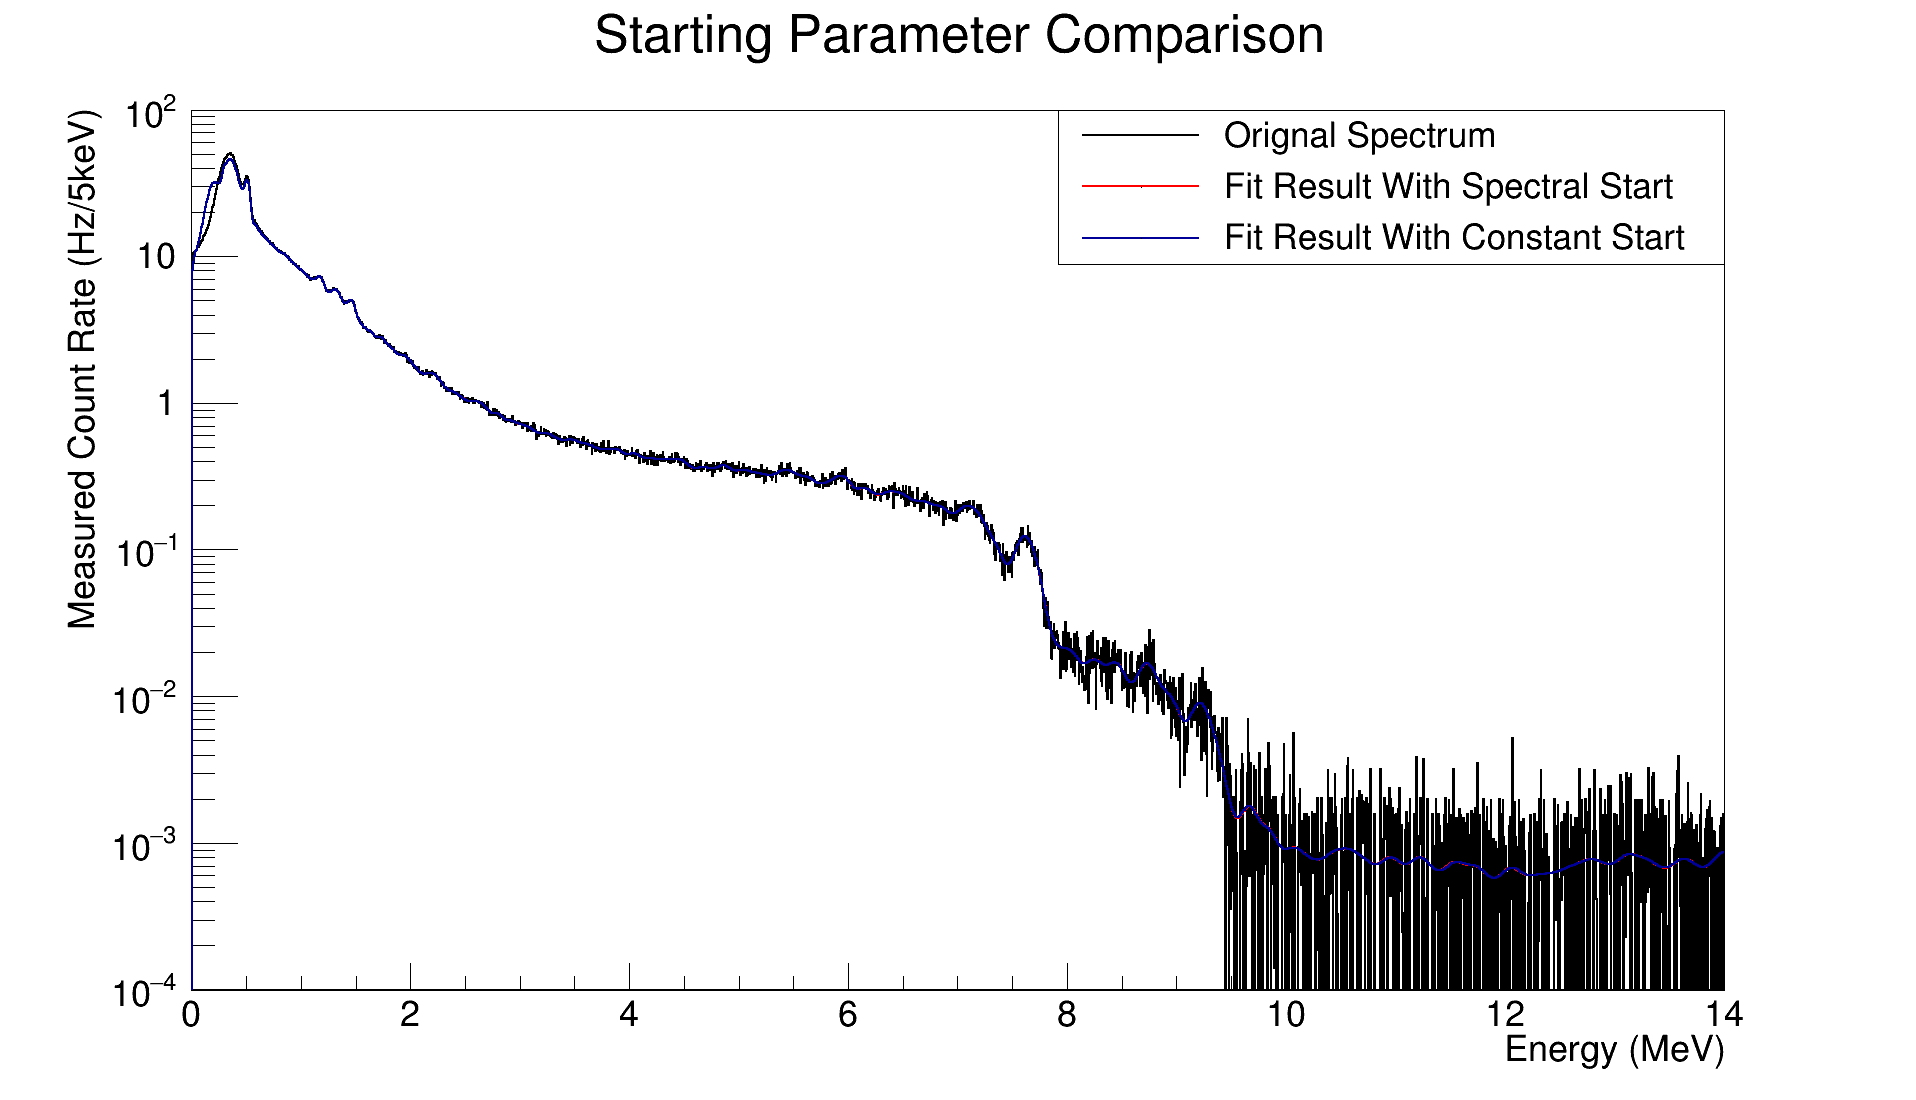
\includegraphics[width=\linewidth]{Start_Fit_Comp_png}
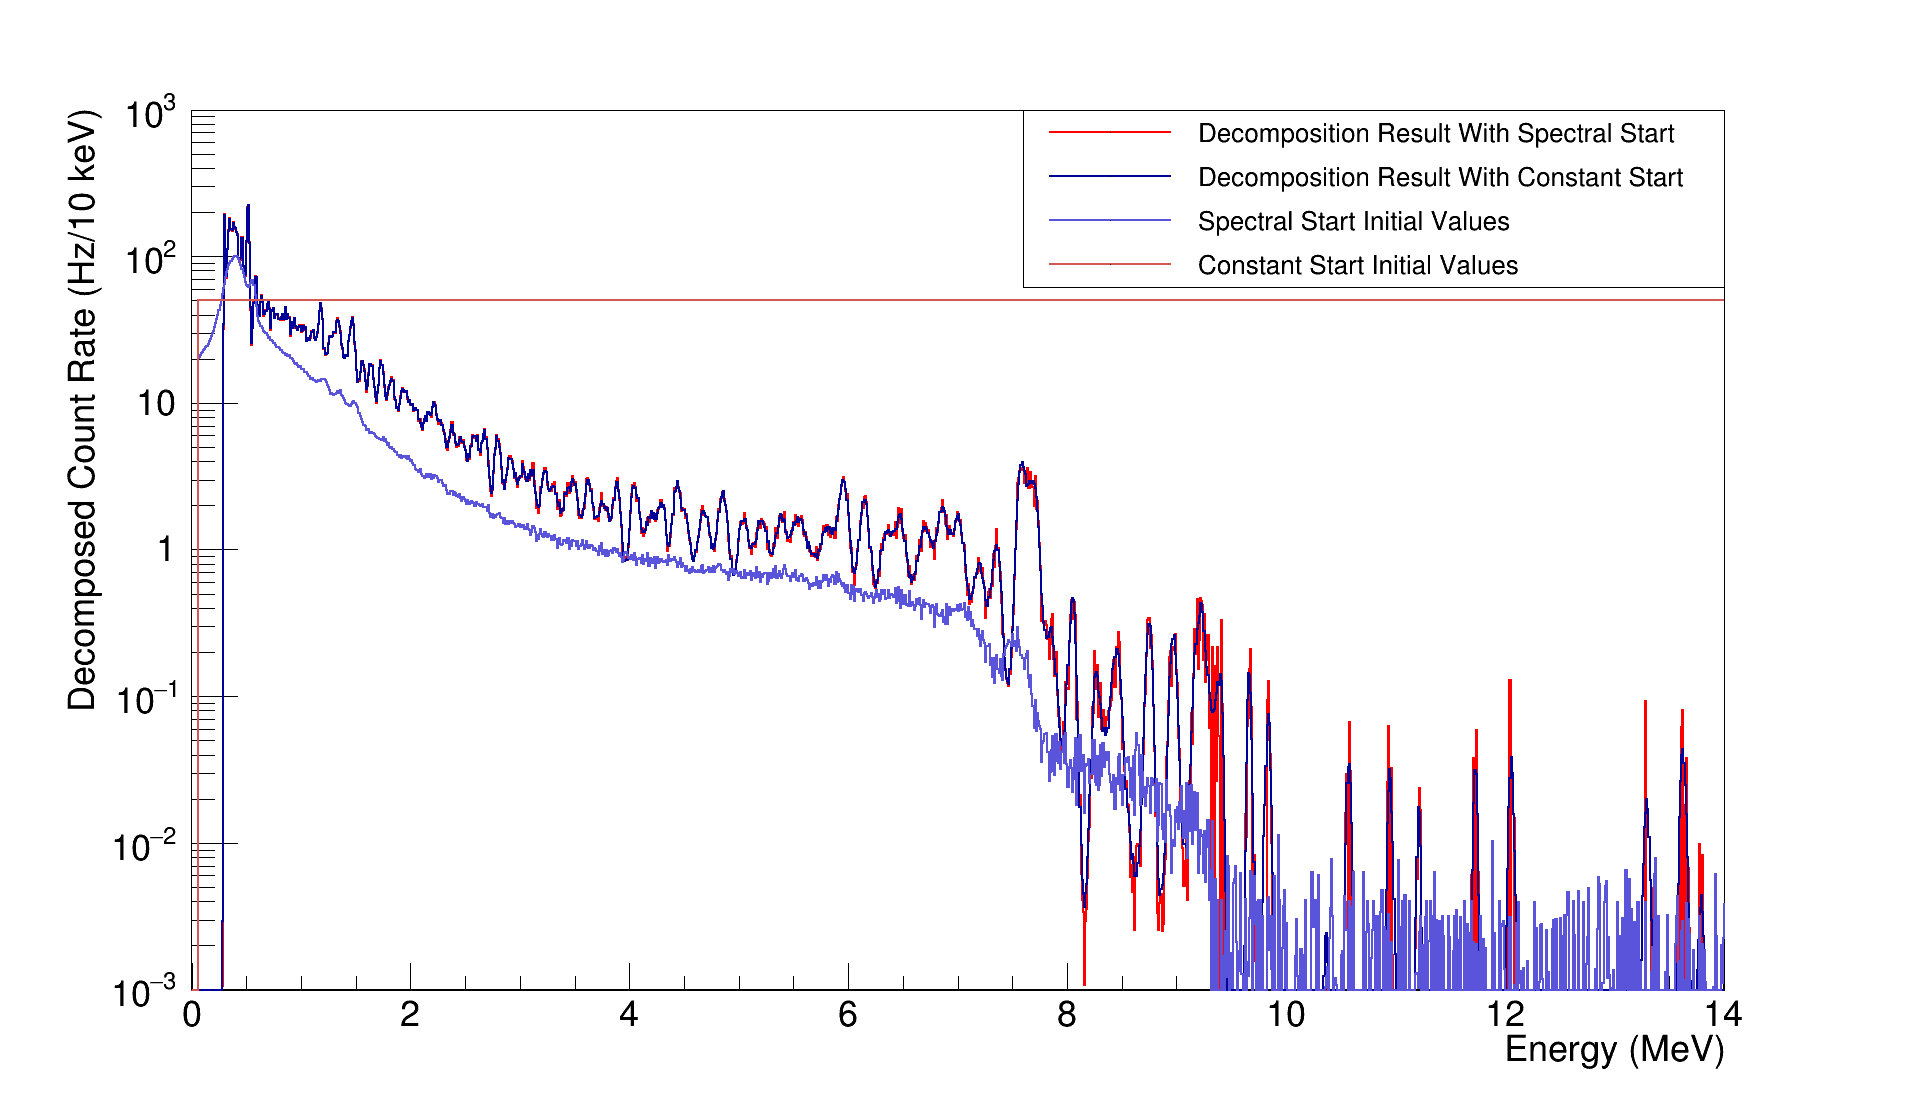
\includegraphics[width=\linewidth]{Start_Decomp_Comp_png}
\caption{(Color Online) Decomposition of the same spectrum from a constant starting}
\label{fig-decomp-starting-pts}
\end{center}
\end{figure}

A final issue is the balance to be struck in the choice of convergence criteria. A choice of parameter change percentage that is too large can result in convergence being declared after too few iterations. Strict choices in general will give good fits; however, if a choice is too strict the resultant fit spectrum will be essentially the same as a fit spectrum with a less strict criterion but will have taken many more iterations to achieve and may have more noise in the incident spectrum. Fig. \ref{fig-convergence-criteria} shows this effect for convergence criteria requiring the fractional difference between two iterations to be less than $0.005$ (which took $1919$ iterations for convergence) and $0.0005$ (which took $23719$ iterations for convergence) with all other parameters being identical ($f^{(0)}_i = 50.0 \forall i$ and not considering values less than $10^{-6}$ for convergence.) In the top panel we see that the fit spectra generated from the two decompositions overlay eachother almost perfectly and overly the input spectrum quite well. In the bottom panel we see that the two decomposition results (the incident spectra) share broadly similar features, but the strict criterion result is much more ``jagged'' likely indicating over-fitting not previously unseen peaks.

\begin{figure}[h]
\begin{center}
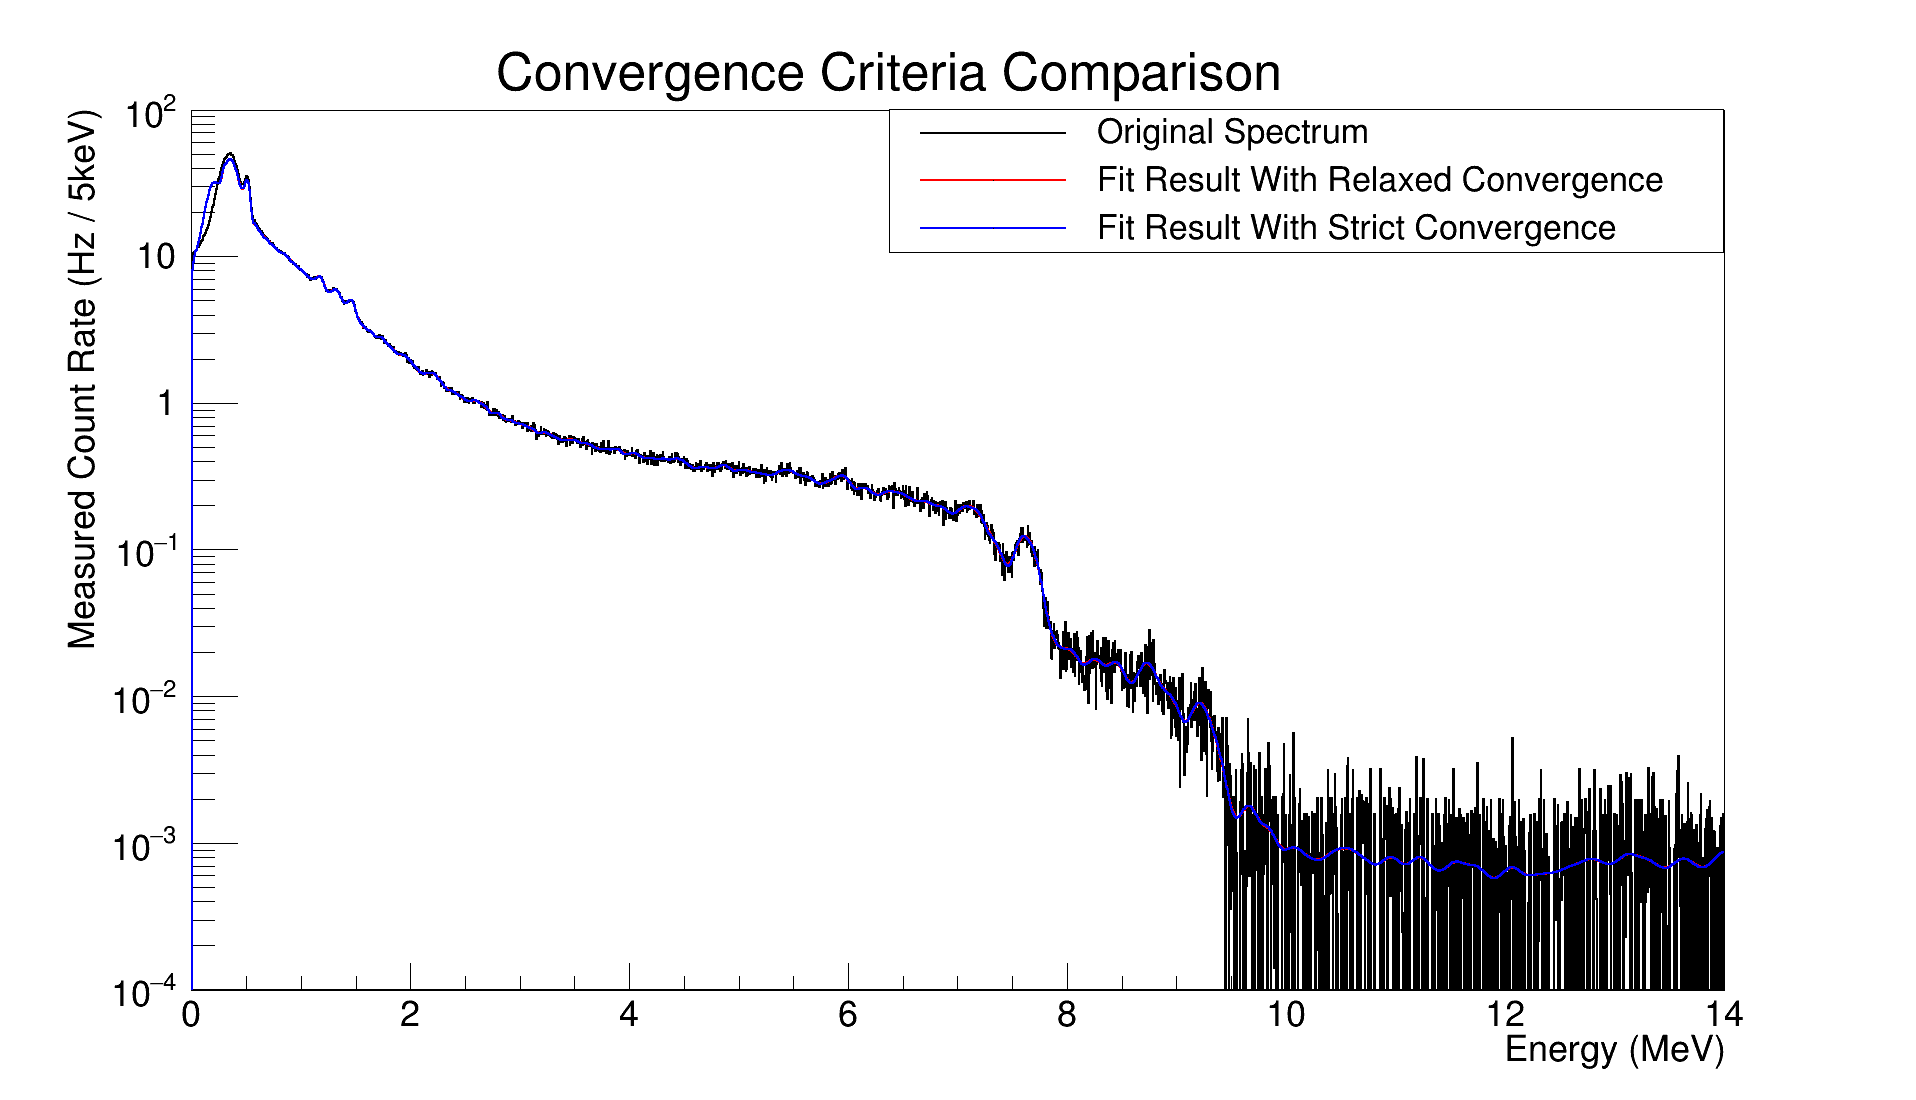
\includegraphics[width=\linewidth]{Conv_Fit_Comp_png}
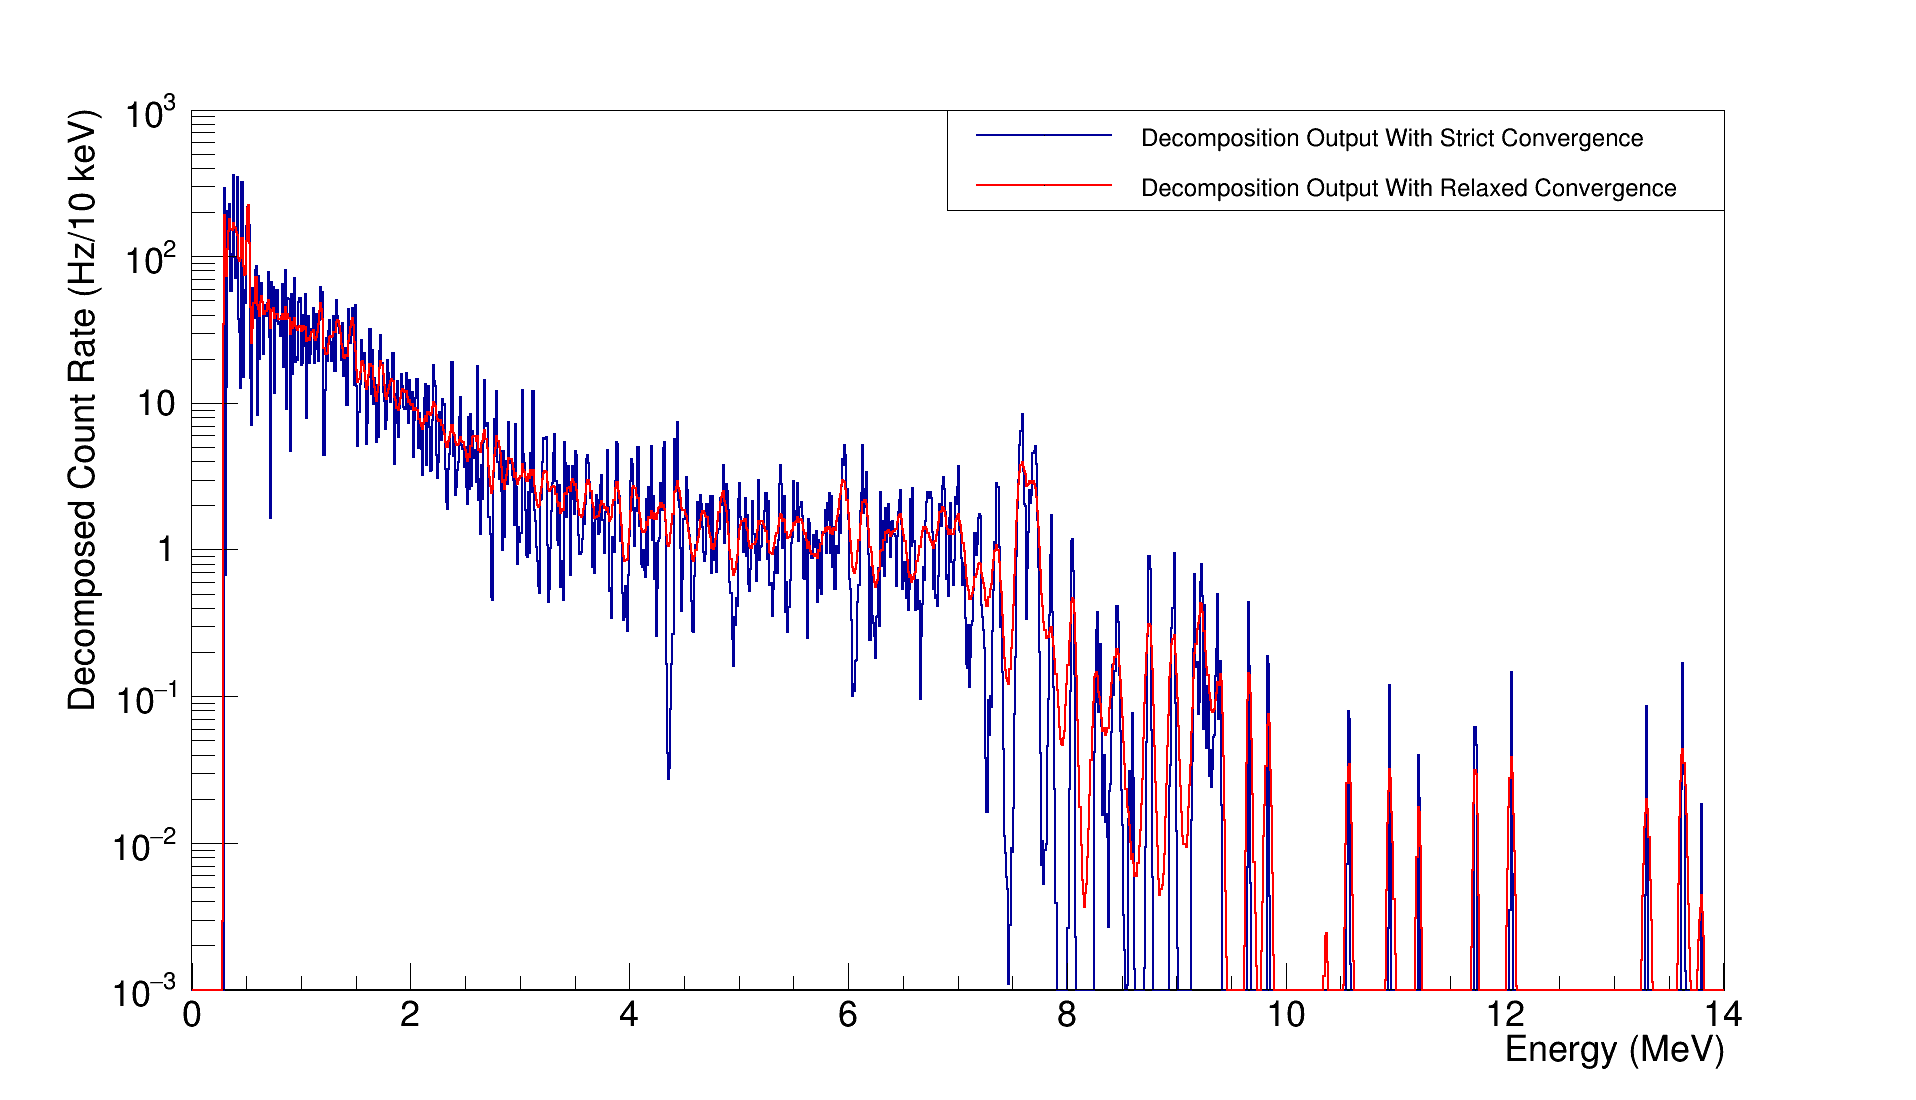
\includegraphics[width=\linewidth]{Conv_Decomp_Comp_png}
\caption{(Color Online) Decomposition of the same spectrum from the same starting point, using a very strict convergence criterion (fractional difference $< 0.0005$)and ``standard'' convergence criterion (fractional difference $< 0.005$).  The strict fit required $23719$ iterations and the standard fit required $1919$ iterations.\emph{Top:} A comparison of the original input spectrum and the resultant fit spectra with the two different convergence criteria. \emph{Bottom:} A comparison of the two decomposition result for both strict and ``standard'' convergence criteria.}
\label{fig-convergence-criteria}
\end{center}
\end{figure}

\subsubsection{Expansions of Usage}

This algorithm also offers an opportunity to solve problems that are not spectrum decomposition. Any problem that can be expressed as finding the set of weights to express a data vector as a weighted sum of other vectors (as in Eqn. \ref{eqn-gen-prob}) can be solved using this algorithm.
\textsc{\begin{align}
d = \sum\limits_{\alpha}f_{\alpha}\times{}\vec{R}_{\alpha}
\label{eqn-gen-prob}
\end{align}}
where $d$ is some data vector, $\vec{R}_{\alpha}$ is a vector in some basis (not necessarily orthogonal) and $f_{\alpha}$ is the weight of the basis vector you wish to extract by fitting (whose final values are positive definite). In this manner you can extract any vector as a linear weighted sum of basis vectors and find the weights. The numerical stability of the algorithm makes it idea for many problems in this form.

To apply this algorithm to an even greater subset of problems satisfying Eqn. \ref{eqn-gen-prob} it is possible, with some care, to relax some of the restrictions on input shown in Alg. \ref{alg_decomp}. While is absolutely certain that $\sum\limits_{j=0}^{m}R_{\mu{}j} > 0$ is necessary, otherwise the first term of Eqn. \ref{eqn-decomposition} will be undefined, other restrictions can be rewritten in somewhat looser forms. So long as values of $f_{\alpha}^{(s)}$ are constrained such that $\sum\limits_{\alpha}R_{\alpha{}i}f_{\alpha}^{(s)} \neq{} 0$, then the $\sum\limits_{j=0}^{n}R_{j\mu{}} > 0$ condition can be relaxed into $\sum\limits_{j=0}^{n}\abs{R_{j\mu{}}} \neq{} 0$ Additionally, so long as care is taken in other places, it is possible to relax the conditions on $f^{(0)}_j$ and $s_j$ to $f^{(0)}_j \neq{0}$ and $\sum\limits_{j=0}^{n}\abs{s_j} > 0$.

\subsubsection{Performance Enhancement}
The algorithm's performance can be substantially improved using the Single Instruction Multiple Data (SIMD) instructions that are present in modern x86 and x86-64 architectures. The SIMD instruction sets allow multiple integer or floating point values to be loaded simultaneously in extra wide registers and then applying an operation to two registers so loaded produces a result that contains multiple values that are the results of adding each of the values in the two input registers pairwise. As all of this is done in the same time required to perform the same sequence using single instruction single data the SIMD instruction sets can offer constant factor speedups ranging from a factor of 2 to 16 depending on the SIMD register size supported by the processor and if single or double precision floating point arithmetic is being used.

\subsection{C++ Implementation}

\lstset{language=C++,
    showspaces=false,
    showtabs=false,
    linewidth=\linewidth{},
    breaklines=false,
    showstringspaces=false,
    breakatwhitespace=false,
    escapeinside={(*@}{@*)},
    commentstyle=\color{green},
    keywordstyle=\color{blue},
    stringstyle=\color{red},
    basicstyle=\ttfamily
}

A header only C++ implementation of this decomposition algorithm has been written and can be found at \url{https://github.com/jmatta1/DecompLib} along with an example demonstrating usage of the library. The library uses templates so that it can be used to work with any floating point type. To use the library one must load a \ic{DataVector} class with the spectrum they wish to decompose, load \ic{DecompVector} class with their initial guess, and load a \ic{RespMat} class with the response matrix they wish to use in the decomposition. Then using their instances of these classes the user invokes \ic{performDecomposition} passing it these instances and, optionally, \ic{MinValue} and \ic{ConvThresh} parameters. \ic{performDecomposition} then uses Alg. \ref{alg_decomp} with $s \gets$\ic{DataVector}, $f^{(0)} \gets$ \ic{DecompVector}, $R \gets$ \\ \ic{RespMat}, $\tau{} \gets$\ic{MinValue}, and $L \gets$\ic{ConvThresh} to perform the decomposition of the spectrum. \ic{performDecomposition} returns either an error code or the number of iterations before convergence was achieved, the result of the decomposition is placed in the \ic{DecompVector}, overwriting the initial parameter set provided by the user.

\section{Conclusions}
In summary: the simulation of response functions for large volume NaI(Tl) detectors has been discussed, a method to decompose spectra using these response functions was shown, pitfalls and opportunities of the decomposition method were listed, and finally a C++ implementation available on GitHub was presented.

\section{Acknowledgements}
The author would like to thank the PROSPECT collaboration for the opportunity to do this work. Additionally, the author would like to thank Charlie Rasco for the many useful discussion about the decomposition algorithm. Finally, the author would like to thank Alfredo Galindo-Uribarri for his support and recommendations over the course of this work. This work is funded in part by DOE \emph{Grant number ...} and a grant from the Heising-Simons Foundation \emph{Grant number}.

\section*{References}
\bibliographystyle{elsarticle-num}

\bibliography{references}

\end{document}